%% Generated by report/build.js -- edit report/content.js, not this file.
%% Figures are emitted as SVG; build.js also writes PDF copies for pdflatex.
\documentclass[conference]{IEEEtran}
\IEEEoverridecommandlockouts
\usepackage{cite}
\usepackage{amsmath,amssymb,amsfonts}
\usepackage{graphicx}
\usepackage{booktabs}
\usepackage{textcomp}
\usepackage{url}

\begin{document}

\title{End-to-End Implementation of a Neuro-Evolutionary Autonomous Navigational System: A Capstone Project in Applied AI}
\author{\IEEEauthorblockN{Deeghayu Suwahas Adhikari, 258722D, MDS\&AI, UoM}
\IEEEauthorblockA{Master of Data Science and Artificial Intelligence, Department of Computer Science and Engineering, Faculty of Engineering, University of Moratuwa\\
Milestone 3 — Final Report}}

\maketitle

\begin{abstract}
This report presents the design, implementation and quantitative evaluation of an autonomous driving controller optimised by neuroevolution and built entirely from first principles: a hand-written multilayer perceptron, a hand-written genetic algorithm, a custom kinematic simulator and a synthetic range sensor, with no machine-learning framework. The environment is a real road topology imported from OpenStreetMap comprising 446 nodes and 1,870 collision boundaries. A headless, seeded evaluation harness that reuses the unmodified simulation sources reveals that the objective function committed at the technical checkpoint was degenerate: the route-progress score returned zero at every location, yielding 1 distinct fitness value across a population of 60 and no improvement over 30 generations, while the running system continued to present every appearance of learning. After repairing the underlying loader-consumer contract mismatch, selection pressure is restored and measurable learning follows. The evolved controller is then compared against three tuned hand-written baselines and a map-privileged pure-pursuit reference on 20 held-out start poses using paired non-parametric tests and bootstrap confidence intervals. Replacing the shipped clone-and-mutate operator with tournament selection and uniform crossover reduces seed-to-seed variance by 3.3 times and improves held-out route progress by a factor of 3.1. An ablation over depth, mutation rate and sensing shows that additional network depth measurably degrades performance, contradicting the direction proposed at the checkpoint. The tuned reactive heuristic nonetheless outperforms the best evolved controller on held-out poses by a factor of 1.8, and the map-privileged reference still collides in 85\% of episodes — establishing both that a hand-written rule is the better engineering choice at this scale, and that a substantial share of the residual failure rate belongs to the vehicle model rather than to any policy.
\end{abstract}

\begin{IEEEkeywords}
Neuroevolution, genetic algorithms, autonomous vehicles, objective specification, silent failure, simulation, reproducibility, comparative evaluation
\end{IEEEkeywords}

\section{Introduction}

\label{sec:intro}

Autonomous driving research is dominated by two kinds of artefact. At one end sit photo-realistic simulators such as CARLA \cite{carla}, which model sensing and dynamics in great detail but present the control problem as a closed box: a student who trains a policy inside one of them learns how to call an API, not how a perception-to-actuation loop is constructed. At the other end sit toy demonstrations on closed oval tracks, where a car that learns to hold a constant steering angle can look competent indefinitely. Neither extreme forces the practitioner to confront the part of the problem that actually decides whether a learned controller works: the quality of the objective it is optimising, and whether the environment is structurally rich enough for that objective to mean anything.

This capstone occupies the space between them. The system is a browser-based two-dimensional driving simulator built from first principles — kinematics, ray-cast range sensing, polygon collision detection, a multilayer perceptron and a genetic algorithm are all hand-written, with no machine-learning framework and no game engine. Its world is not a hand-drawn oval but a real road topology imported from OpenStreetMap \cite{osm}: 446 nodes and 472 centreline segments, expanded into 1,870 collision boundaries across a 16,542 x 9,608 pixel extent. Because every layer is visible, the failure modes are visible too.

That transparency turned out to matter more than expected. The central empirical finding of this report is not that neuroevolution works — it does, and the numbers below quantify how well — but that the version of the system submitted at the Milestone 2 technical checkpoint \textbf{could not learn at all}, for a reason that no amount of watching the simulator run would have revealed. The route-progress objective driving the genetic algorithm returned exactly zero at every location in the world. Every individual in every generation tied. Selection was a coin flip, and the visible behaviour — cars driving, dying, respawning, a generation counter incrementing, a live network visualiser animating — was indistinguishable from learning. It took a measurement harness, not a demonstration, to find it.

\subsection{Problem statement}

\label{sec:problem}

The problem addressed is the \emph{evaluation} of neuroevolutionary control strategies for autonomous driving in structurally complex road topologies. Concretely: given a vehicle with a five-beam range sensor and four binary actuators, operating on a real urban road graph, how far can a neural controller evolved by a genetic algorithm travel along the road network before failing, and how does that compare against hand-written geometric controllers given the same sensing and the same actuators?

The question is deliberately comparative. A neuroevolutionary result reported on its own is uninterpretable: without a baseline, a policy that survives twenty seconds could be a sophisticated navigator or a car driving in a large circle. The Milestone 1 project definition committed to exactly this comparison — an evolved network against a rule-based heuristic — and this report delivers it, together with the reference ceiling supplied by a controller that is allowed to see the map.

\subsection{Contributions}

\label{sec:contributions}

\begin{itemize}
\item \textbf{An end-to-end system}, from OpenStreetMap ingestion through geometric world construction, synthetic range sensing, hand-written neural inference and evolutionary optimisation, to quantitative evaluation — with no machine-learning dependencies of any kind.
\item \textbf{A reproducible headless evaluation harness} that loads the unmodified browser simulation sources into a Node.js context, installs a seeded pseudo-random generator in place of \texttt{Math.random}, and replays episodes deterministically. Approximately 86,400 training and evaluation episodes underpin the results reported here.
\item \textbf{A diagnosed and repaired silent failure} in the fitness signal, with a controlled measurement of its cost: the as-committed objective produced 1 distinct fitness value across a population of 60, against 27 for the repaired one.
\item \textbf{Four tuned baselines} — a random network, a reactive finite-state heuristic, a proportional steering controller and a map-privileged pure-pursuit reference — each grid-searched on validation poses so that the comparison is not a straw man.
\item \textbf{A held-out generalisation protocol.} Training happens from a single start pose, exactly as the interactive system does; evaluation happens on 20 start poses drawn from elsewhere in the road graph and never seen during training or tuning.
\item \textbf{An ablation study} over network depth, mutation rate, sensor count and sensor range, whose architecture result contradicts the direction the Milestone 2 checkpoint proposed to take.
\end{itemize}

\subsection{Structure of this report}

\label{sec:structure}

Section~\ref{sec:related} positions the work against the neuroevolution and simulation literature. Section~\ref{sec:scope} states the bounded scope choices and the research questions. Section~\ref{sec:data} covers data sourcing, geometric engineering and data quality. Section~\ref{sec:system} and Section~\ref{sec:method} describe the system and the learning algorithm. Section~\ref{sec:baselines} and Section~\ref{sec:protocol} describe what the learned agent is measured against and how. Section~\ref{sec:results} presents the results, Section~\ref{sec:discussion} interprets them, and Section~\ref{sec:limitations} states the limitations and trade-offs. Appendix A is the required reproducibility checklist; Appendix C records corrections to the earlier submissions.

\begin{figure*}[!t]
\centering

\includegraphics[width=\textwidth]{figures/fig_architecture}
\caption{End-to-end pipeline. Geospatial data is compiled into a drivable world and a Dijkstra route-progress field; the vehicle senses that world through simulated range beams, a multilayer perceptron converts the readings into four actuator bits, and a genetic algorithm selects over the resulting behaviour. Measurement is deliberately kept separate from the training signal.}
\label{fig:arch}
\end{figure*}

\section{Background and Related Work}

\label{sec:related}

\subsection{Neuroevolution as an alternative to gradient methods}

Neuroevolution optimises the weights, and sometimes the topology, of a neural network with an evolutionary algorithm rather than by gradient descent \cite{holland,neat}. Its appeal in control is structural: the objective need not be differentiable, and no labelled trajectories are required. In sequential decision problems the reward is typically sparse and delayed — a vehicle either completes a manoeuvre or does not — which is precisely the regime where backpropagation has nothing to propagate without an intermediate value function to manufacture one.

The practical viability of the approach at scale was demonstrated by Salimans et al., who showed that a simple evolution strategy is competitive with policy-gradient reinforcement learning on standard control benchmarks while parallelising almost perfectly \cite{es}. Koutník et al. had earlier evolved recurrent controllers with over a million weights for vision-based driving in TORCS \cite{koutnik}. Stanley and Miikkulainen's NEAT introduced topology evolution with historical markings and speciation \cite{neat}; the present work uses a fixed topology, a deliberate simplification whose consequences are discussed in Section~\ref{sec:limitations}. End-to-end supervised imitation \cite{bojarski} represents the alternative paradigm, and is excluded here precisely because it requires demonstration data that this project has no way to obtain.

\subsection{Objective specification and deception}

The dominant failure mode of evolutionary control is not slow convergence but a badly specified objective. Lehman and Stanley's work on deception showed that an objective function can \emph{actively} misdirect search toward dead ends, and that abandoning the objective in favour of behavioural novelty often solves deceptive problems more reliably \cite{novelty}. The wider literature on specification gaming and reward misspecification makes the same point from the safety side \cite{amodei}.

This report contributes an extreme and instructive case: an objective that is not deceptive but \emph{degenerate}. It does not point the search in a wrong direction; it points nowhere at all, because it is constant. The distinction matters diagnostically. A deceptive objective produces confident, wrong behaviour that improves on its own terms and is therefore detectable by inspecting what the agent learned. A degenerate one produces a flat learning curve, a population whose fitness values are identical, and a system that still \emph{looks} like it is training. Sculley et al.'s catalogue of hidden technical debt in machine-learning systems anticipates exactly this class of fault: the entanglement of a data loader with a downstream consumer that silently assumes a field the loader never populates \cite{sculley}.

\subsection{Simulation platforms and the transparency trade-off}

CARLA \cite{carla} and comparable platforms provide validated dynamics, sensor models and traffic scenarios. The cost is opacity: a result obtained inside such a simulator is conditional on modelling decisions the experimenter cannot inspect, and the sim-to-real gap is addressed by techniques such as domain randomisation \cite{tobin} that presuppose control over the very parameters a closed simulator hides. Building the simulator from scratch inverts the trade: fidelity is much lower, but every assumption is auditable and every failure is attributable. Given that the research question here concerns the \emph{optimisation process} rather than physical realism, that is the correct side of the trade to be on — a position made concrete by the fact that the defect reported in Section~\ref{sec:results} would have been invisible behind a simulator API.

\subsection{Evaluation methodology in evolutionary and reinforcement learning}

A recurring criticism of empirical work in this area is that results are reported from a single run, on the conditions the method was developed against, without a competitive baseline. Each of those three omissions is individually sufficient to make a result unfalsifiable, and together they describe the Milestone 2 draft of this project accurately. The protocol adopted here is a direct response: multiple independent seeds with dispersion reported rather than a single champion; a train/validation/test split over initial conditions; baselines tuned on the validation split so that the comparison is not decided by how much effort each side received; and rank-based tests with effect sizes rather than means alone.

Two methodological choices deserve explicit defence because they are less common. First, the primary metric is computed with an instrument that is independent of the training signal: an arm trained on a broken objective is still scored on a working one. Without this, an arm cannot be compared against another that optimised something different, and the central experiment of this report would have been impossible to state. Second, a \emph{privileged} reference controller is included. Reporting a learned agent's collision rate without knowing what a controller with perfect map knowledge achieves on the same plant invites the reader to attribute the entire residual to the policy; Section~\ref{sec:results} shows that attribution would have been wrong by a wide margin.

\subsection{Geometric baselines}

Pure pursuit \cite{coulter} remains the standard geometric path-tracking baseline: it selects a goal point a fixed look-ahead distance along a reference path and computes the curvature that reaches it. It requires the path, which a learned agent operating on raw range readings does not have, so in this study it serves as a privileged upper reference rather than as a competing method. Reactive wall-following and proportional steering on sensor asymmetry are the classical non-privileged heuristics, and both are implemented and tuned here.

\section{Problem Definition and Scope}

\label{sec:scope}

\subsection{Bounded scope choices}

Following the capstone's scoping framework, the project is defined by four explicit choices, unchanged from the Milestone 1 definition:

\begin{itemize}
\item \textbf{Problem type — control and optimisation.} The system emits actuation commands to maximise an objective, rather than predicting a label.
\item \textbf{Data type — graph and synthetic sensor data.} The environment is a geospatial graph (OpenStreetMap nodes and ways); the agent observes only synthetic range readings derived from ray casting against that geometry.
\item \textbf{Technique category — neuroevolution.} A fixed-topology multilayer perceptron whose weights are optimised by a genetic algorithm.
\item \textbf{System context — comparative analysis.} The deliverable is a testbed producing empirical comparisons between control strategies, not a deployed product.
\end{itemize}

No external large language model is used anywhere in the pipeline, so the capstone's requirements governing LLM-based projects do not apply to this submission.

\subsection{Research questions}

\begin{itemize}
\item \textbf{RQ1.} Does the route-progress objective as committed at the technical checkpoint provide usable selection pressure?
\item \textbf{RQ2.} How much does the choice of fitness definition — degenerate route progress, Euclidean displacement, or corrected route progress — change what is learned?
\item \textbf{RQ3.} Does replacing the shipped clone-and-mutate reproduction operator with tournament selection and uniform crossover improve final performance, its variance, or neither?
\item \textbf{RQ4.} How does the best evolved controller compare with tuned rule-based baselines and with a map-privileged reference on start poses never seen during training?
\item \textbf{RQ5.} Which design choices — network depth, mutation rate, sensor count, sensor range — actually matter?
\end{itemize}

\subsection{Success criteria}

The project succeeds if it produces a working end-to-end pipeline, a statistically defensible comparison against at least one non-trivial baseline, and an honest account of where the approach fails. Reaching a particular route-progress figure is explicitly \emph{not} a success criterion, because the appropriate figure is unknown a priori; the pure-pursuit reference exists to supply that missing context.

\section{Data: Sources, Engineering and Quality}

\label{sec:data}

\subsection{Source and provenance}

The world derives from OpenStreetMap \cite{osm}. Node coordinates and way geometry were extracted through the Overpass API, projected into a planar pixel coordinate system, and serialised into a single JavaScript module of 6.1 MB (\texttt{simulation/simulationData.js}, 6,367,313 bytes) that the browser loads directly. Deserialisation into live geometry takes 188 ms. Committing the extract to the repository rather than querying Overpass at run time is a deliberate reproducibility decision: Overpass responses vary with server state and with subsequent edits to the map, so a live query would make the experiments unrepeatable.

The second data source is entirely synthetic and generated online: the range readings produced by casting rays from the vehicle against the road boundary geometry. These are the only observations any learned policy in this study ever receives.

\subsection{From a road graph to a drivable world}

The centreline graph alone is not drivable — it has no width, no boundaries and nothing to collide with. The world builder performs three geometric transformations. First, each centreline segment is expanded into an \emph{envelope}: a rounded rectangle of width 100 px, generated by sweeping 10 points around each endpoint. Second, the envelope polygons are combined by a boolean union that splits every pair of intersecting edges at their intersection point and discards edges lying inside another polygon; what survives is the outline of the road surface. Third, that outline becomes the 1,870 line segments used for both ray casting and collision detection. Buildings and trees are generated procedurally outside the road envelope (433 and 500 respectively); they are rendered but are not collidable, a modelling limitation recorded in Section~\ref{sec:limitations}.

\begin{figure*}[!t]
\centering

\includegraphics[width=\textwidth]{figures/fig_map}
\caption{The ingested road network. Grey fills are generated building footprints; the large marker is the single start pose used for all training, and the smaller markers are the held-out poses used for evaluation. The topology contains loops, T-junctions, cul-de-sacs and four-way intersections rather than a closed circuit.}
\label{fig:map}
\end{figure*}

\subsection{Descriptive statistics}

Table~\ref{tab:data} summarises the ingested world. Two properties dominate the difficulty of the control task. First, segment lengths are extremely heterogeneous: a median of 99 px against a mean of 215 px and a maximum of 1,453 px, so a single policy must handle both long straight runs and dense clusters of short segments at junctions. Second, the road half-width is 50 px while the vehicle is 30 x 50 px and the steering resolution is a fixed 0.07 rad per frame, which leaves very little lateral margin through a tight corner.

\begin{table}[!t]
\caption{Descriptive statistics of the ingested world}
\label{tab:data}
\centering
\footnotesize
\begin{tabular}{lr}
\toprule
Property & Value \\
\midrule
\multicolumn{2}{l}{\emph{Road graph}} \\
Nodes & 446 \\
Centreline segments & 472 \\
Connected components & 3 \\
Largest component & 428 nodes (96.0\%) \\
Nodes of degree 1 / 2 / 3 / 4 & 20 / 369 / 42 / 15 \\
Reachable from start pose & 428 / 446 (96.0\%) \\
Longest route distance from start & 17,822 px \\
\multicolumn{2}{l}{\emph{Segment length (px)}} \\
Minimum / median / maximum & 10 / 99 / 1,453 \\
Mean ± SD & 215 ± 255 \\
Interquartile range & 62 – 248 \\
\multicolumn{2}{l}{\emph{Derived geometry}} \\
Road boundary segments & 1,870 \\
Lane guides & 2,112 \\
Building footprints (non-collidable) & 433 \\
Trees (non-collidable) & 500 \\
Road width / half-width (px) & 100 / 50 \\
\multicolumn{2}{l}{\emph{Extent and annotation}} \\
Bounding box (px) & 16,542 × 9,608 \\
Semantic markings & 1 (start) \\
One-way segments & 149 \\
\bottomrule
\end{tabular}
\\[2pt]\parbox{\linewidth}{\scriptsize Generated by \texttt{experiments/datasetStats.js}; the full record is \texttt{experiments/results/dataset\_stats.json}.}
\end{table}

\begin{figure*}[!t]
\centering

\includegraphics[width=\textwidth]{figures/fig_data}
\caption{Node degree distribution of the road graph. Degree-2 nodes represent ordinary road curvature; degree-1 nodes are dead ends the agent can enter and never escape; degree 3 and 4 are the junctions where the ambiguity of an undirected route-progress field becomes acute.}
\label{fig:degree}
\end{figure*}

\subsection{Data quality problems and how they were handled}

Three quality problems in the extract are worth recording, because each has a direct consequence for the experiments.

\textbf{Disconnected components.} The graph is not connected: it decomposes into 3 components of sizes 428, 13, 5. Only 96.0\% of nodes lie in the largest component. Nodes outside it are unreachable from the start pose and receive infinite route distance. This is handled explicitly: the scorer treats non-finite distances as unusable, and the held-out pose sampler excludes any pose whose route distance is not finite, so no evaluation episode begins in an unreachable island.

\textbf{Degenerate boundary segments.} The polygon union produces boundary segments as short as 1.3e-5 px — numerically zero-length edges left over from intersection splitting. They are harmless for collision detection, because the intersection routine rejects near-parallel configurations with an epsilon of 0.001, but they inflate the boundary count and therefore the cost of every ray cast, which motivated the spatial index described in Section~\ref{sec:system}.

\textbf{Sparse semantic annotation, and attributes discarded on load.} The extract carries exactly 1 semantic marking — a single start marking. The codebase implements traffic lights, stop lines, yield markings, zebra crossings, parking bays and target nodes, and none of them are exercised by this map. The report therefore makes no claim about traffic-rule compliance: the task studied here is boundary-respecting navigation on an unsignalised network, and describing it as anything more would overstate the evidence.

Directional information tells a different story. The map file does carry direction data — 149 of the 472 centreline segments are tagged one-way — but the graph loader discarded that tag on deserialisation, so until the repair described in Section~\ref{sec:results} the route field treated every street as bidirectional. This is the same class of fault as the one that disabled the objective, found in the same function, and it is recorded here because it shows the defect was not an isolated slip: the loader dropped every attribute the geometry constructor did not name.

A fourth issue — the loss of node identity during deserialisation — is not merely a data quality problem but the root cause of the central experimental finding, and is treated in full in Section~\ref{sec:results}.

\subsection{Coordinate system and units}

All geometry is expressed in a planar pixel space rather than in metres or in geographic coordinates. The extract was projected once, offline, and the projection is not inverted anywhere in the running system, so no result in this report is expressed in real-world units. This is a deliberate simplification with two consequences worth stating. It means the vehicle's 30 × 50 px footprint and the road's 100 px width are internally consistent but carry no metric interpretation; and it means the speed values, which the interface displays as kilometres per hour by multiplying by ten, are a presentational convenience with no physical grounding. Wherever this report quotes a speed it does so in simulator units.

Working in pixel space also avoids a class of error the project would otherwise have had to manage: with a spherical projection, Euclidean edge weights in the Dijkstra field would be wrong by a latitude-dependent factor, and the ray-segment intersection test would need to operate on a curved surface. Since the research question concerns the optimiser and not geodesy, discarding the geographic frame removes complexity that would buy nothing.

\subsection{Splits: what counts as held out}

Supervised learning splits rows; a control problem has no rows to split, so the split must be over \emph{initial conditions}. Three disjoint sets of start poses are used:

\begin{itemize}
\item \textbf{Training condition (n = 1).} The single start marking present in the map. All evolutionary runs begin here, mirroring exactly what the interactive browser system does.
\item \textbf{Validation poses (n = 10).} Used to tune the rule-based baselines and to select among ablation variants. Never used for any reported comparison.
\item \textbf{Test poses (n = 20).} Used once, for the final comparison in Section~\ref{sec:results}. Never used for tuning or model selection.
\end{itemize}

Poses are sampled deterministically: nodes of degree at least two whose route distance from the start is finite are shuffled with a fixed seed (2026 exclusive-ORed with 0x5eed) and split into the validation and test sets, with the heading taken along one incident segment. Because the seed is fixed, the split is reproducible from the code alone. Each pose additionally carries its own Dijkstra field rooted at that pose, so route progress measured from a held-out start is progress relative to \emph{that} start rather than to the training origin.

\subsection{Feature construction}

The observation vector is constructed identically for every controller studied. Each of the five beams returns either no hit, or the intersection nearest the vehicle expressed as a normalised offset t in [0, 1] along the beam. The feature is 1 − t, so a value of 0 means clear to the sensor's full range and a value approaching 1 means an obstacle against the bumper. A missing return is encoded as 0. No further scaling, whitening or temporal history is applied: the policy is purely reactive and memoryless, a modelling choice whose consequences are examined in Section~\ref{sec:discussion}.

\section{System Architecture}

\label{sec:system}

\subsection{Overview}

Fig.~\ref{fig:arch} shows the pipeline. The three vertical bands are, from left to right, data engineering (geospatial ingestion, geometric world construction, route-progress field), simulation (range sensing, policy inference, kinematics), and learning plus measurement (fitness, genetic algorithm, evaluation). The separation of the measurement band from the learning band is deliberate and is justified in Section~\ref{sec:protocol}.

\subsection{Perception: simulated range sensing}

The sensor is an array of five rays fanned across a π/2 field of view centred on the vehicle's heading, each 220 px long. For each ray the module computes the intersection with every nearby boundary segment and with the edges of any traffic polygon, and keeps the nearest. The test is the standard parametric line-segment formulation: for ray \emph{AB} and segment \emph{CD},

\begin{equation}
t = \frac{(x_D-x_C)(y_A-y_C)-(y_D-y_C)(x_A-x_C)}{(y_D-y_C)(x_B-x_A)-(x_D-x_C)(y_B-y_A)}
\end{equation}

with the analogous expression for the second parameter u, and a hit recorded only when both lie in [0, 1]. A denominator smaller than 0.001 in absolute value is rejected as parallel. The returned t is exactly the normalised distance used as a network input, so no separate distance computation is required.

Fig.~\ref{fig:lidar} shows the sensor operating at a five-way junction, which is the hardest class of situation in this map. Two properties of the representation are visible. First, the beams terminate on the road boundary and nowhere else — buildings and trees are drawn but are not in the collision set, so the agent is blind to them. Second, at a junction most beams return no hit at all and are therefore encoded as 0, which is the same value as a boundary at maximum range. The agent consequently cannot distinguish "open space ahead" from "nothing within 220 px", and it is precisely at junctions that this ambiguity bites.

\begin{figure}[!t]
\centering
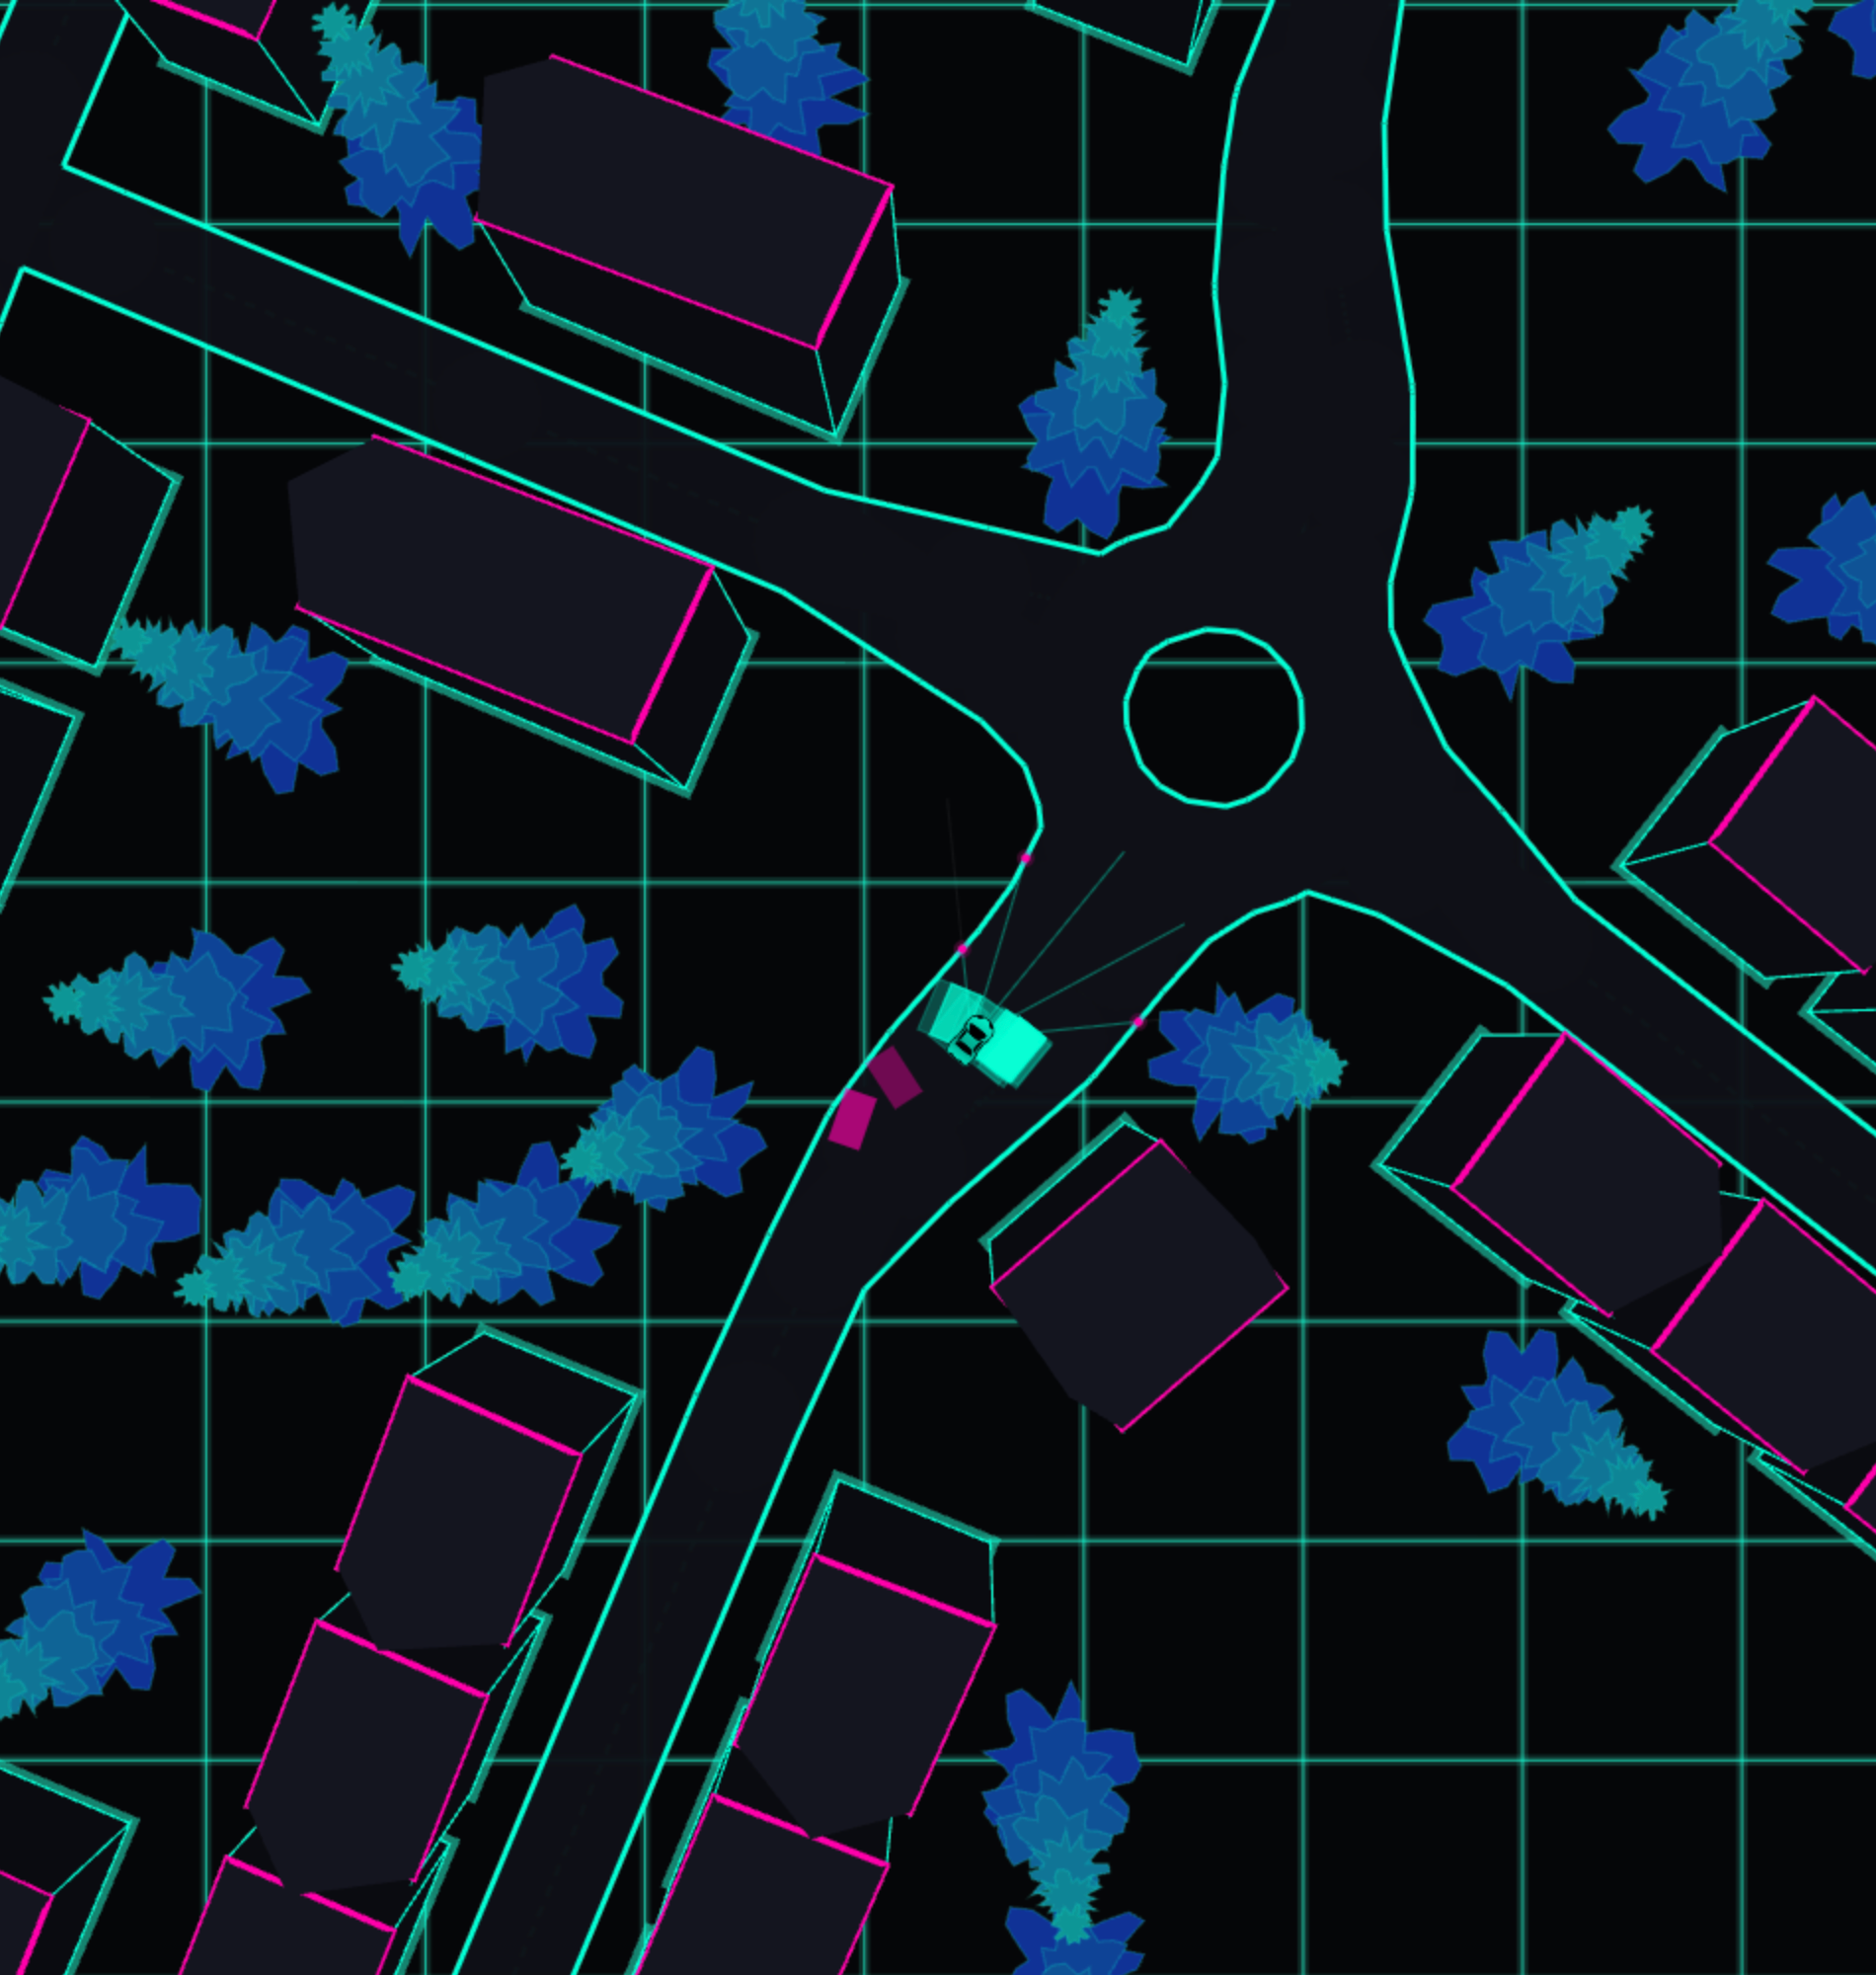
\includegraphics[width=\columnwidth]{figures/lidar_closeup.png}
\caption{The range sensor at a five-way junction. The lead vehicle casts five beams across a pi/2 field of view; small markers show where a beam meets a road boundary. The magenta bodies behind it are swarm members already eliminated in this generation. Building and tree geometry is rendered but is not collidable and returns no beam hits.}
\label{fig:lidar}
\end{figure}

\subsection{Vehicle kinematics}

The vehicle model is a \emph{unicycle} with speed-coupled steering, not a bicycle model. This correction matters, because the Milestone 2 draft described it as a kinematic bicycle model; there is no wheelbase parameter and no steering-angle state anywhere in the implementation. The update, executed once per frame, is: apply throttle and brake to the scalar speed, clip it, apply friction, rotate the heading only if the vehicle is moving, and translate along the new heading.

\begin{equation}
\theta_{t+1} = \theta_t + \delta\,\mathrm{sgn}(v_{t+1})\,\big(u_{\mathrm{left}}-u_{\mathrm{right}}\big)
\end{equation}

\begin{equation}
x_{t+1} = x_t - v_{t+1}\sin\theta_{t+1}, \qquad y_{t+1} = y_t - v_{t+1}\cos\theta_{t+1}
\end{equation}

with acceleration 0.2, friction 0.05, steering increment δ = 0.07 rad, forward speed capped at 6 and reverse at half that. The multiplication of the steering increment by sgn(v) is the single most consequential modelling decision in the simulator: a stationary vehicle cannot rotate, so any policy must learn that turning requires committing to speed. It also means the heading is not independently controllable, which bounds how tightly \emph{any} controller — learned or hand-written — can corner.

\subsection{Collision model}

The vehicle is represented as a rotated rectangle reconstructed each frame from its centre, heading and dimensions. Damage is declared when any edge of that rectangle intersects any road boundary segment or any edge of a traffic polygon. Collision is terminal: there is no damage accumulation and no recovery, so an episode ends at first contact. This makes collision a clean binary event for measurement, at the cost of not modelling glancing contacts or recoverable scrapes.

\subsection{Policy network}

The controller is a fixed-topology multilayer perceptron with layer widths 5–12–10–4, giving 246 trainable parameters. Each layer computes a weighted sum, adds a bias, applies a logistic function and thresholds it:

\begin{equation}
a^{(l)}_j = \mathbb{1}\Big[\sigma\Big(\textstyle\sum_i w^{(l)}_{ij} a^{(l-1)}_i + b^{(l)}_j\Big) > 0.5\Big]
\end{equation}

Because σ(z) > 0.5 exactly when z > 0, the logistic function is computationally redundant: the network is a stack of linear threshold units — a hard-threshold perceptron network. This is worth stating plainly rather than describing the architecture as having a sigmoid activation, because it explains a result in Section~\ref{sec:results}. With binary activations, hidden layers can only realise threshold functions of threshold functions, and the effective hypothesis class grows far more slowly with depth than the parameter count suggests. It also means gradients do not exist anywhere in the network, which is precisely why a gradient-free optimiser is the appropriate choice rather than merely an aesthetic one.

The four outputs map to forward, left, right and reverse. Conflicts are resolved before actuation: simultaneous left and right cancel to straight, and forward dominates reverse.

\subsection{Route-progress field}

Progress along the road network is measured with a single-source shortest-path field. Dijkstra's algorithm \cite{dijkstra} runs over the centreline graph from the node nearest the start pose with Euclidean edge weights, assigning each node a route distance. The score at an arbitrary vehicle position is obtained by projecting the position onto the nearest centreline segment and linearly interpolating the two endpoint distances by the projection parameter. The field is computed once per pose and reused for every episode; the longest route distance in this map is 17,822 px.

It is important to be precise about what this quantity is. It is a \emph{radial potential}: distance from the origin along the road network, increasing in every direction away from the start. It is not a directed route to a goal. A vehicle that drives away from the origin along any branch scores well, and two branches leading to entirely different places are indistinguishable. This property is exploited by the agents and is analysed in Section~\ref{sec:discussion}.

\subsection{Evaluation harness}

All experiments run headlessly in Node.js. The harness loads the unmodified browser source files — geometry, world construction, route scorer, network, sensor, actuator and vehicle — into a single \texttt{vm} context, supplying minimal stand-ins for the handful of DOM objects that constructors touch. The physics, sensing and inference exercised by every experiment are therefore the same code that runs in the browser; only rendering and the animation-frame driver are replaced. Controller output is hoisted out of the vehicle's update method so that rule-based and learned policies share one code path and therefore identical timing, sensing and termination semantics.

One optimisation was necessary to make batch evaluation tractable. The interactive engine culls boundary segments with a linear scan at an 800 px radius on every frame, which is negligible for one frame but dominates a run of tens of thousands of episodes. The harness pre-buckets the boundary segments into a uniform grid of 256 px cells and answers per-vehicle queries at a 400 px radius. Since 400 px strictly exceeds the 220 px beam length plus the 58 px vehicle diagonal, no segment that could be hit by a ray or by the body is ever discarded, so the optimisation is behaviour-preserving rather than an approximation.

\subsection{Verifying the harness}

A measurement instrument that is itself unverified cannot support the claims made in Section~\ref{sec:results}, so three properties are asserted empirically rather than argued. The script \texttt{experiments/verifyHarness.js} checks them and writes its verdict to \texttt{experiments/results/verification.json}.

\begin{itemize}
\item \textbf{Episode determinism.} The same seed replayed 3 times produces a bit-identical episode signature — frame count, termination cause, peak route progress, path length, net displacement, RMS jerk and mean lateral deviation, each to nine decimal places. Result: pass.
\item \textbf{Culling equivalence.} The claim that the spatial index is behaviour-preserving rather than an approximation is tested directly: each of 8 episodes is run twice from the same genome and seed, once with the 400 px grid query and once with a grid whose single cell spans the entire world, which returns every boundary segment. Result: 8 of 8 trajectory signatures identical. The geometric argument — that a 400 px radius strictly exceeds the 220 px beam plus the 58 px vehicle diagonal — is therefore confirmed by measurement and not merely asserted.
\item \textbf{Training determinism.} Two independent invocations of the evolutionary loop under one seed produce byte-identical fitness histories across all generations. Result: pass.
\end{itemize}

These checks are cheap, run in seconds, and are the reason the numbers in this report can be regenerated exactly rather than approximately. They do not verify that the harness matches the browser build's \emph{rendering}, which is irrelevant, nor that the physics is realistic, which it is not; they verify that the instrument returns the same reading twice and that the one optimisation applied to it changes nothing.

\subsection{The interactive application}

The evaluation harness is one of two front-ends onto the same simulation core; the other is the browser application that constitutes the delivered system. It is a single-page application with no build step and no dependencies: \texttt{index.html} loads seventeen plain scripts in dependency order and the simulation starts on the load event. Four surfaces are rendered each frame.

\begin{itemize}
\item \textbf{The world canvas}, drawn in a camera space that follows the current leader. Road envelopes, boundaries, buildings and trees are drawn with a fake-3D projection that offsets each vertex away from the view point in proportion to \texttt{atan(d/300)}, giving parallax without a 3D pipeline. Rendering is culled to a 1500 px radius around the view point.
\item \textbf{A neural visualiser} that draws the champion's network live, with connection thickness encoding the magnitude of the weight \emph{change} since the start of the generation rather than the weight itself, so the display shows what evolution is doing rather than what the network currently is. Positive weights are drawn in one hue and negative in another, node fill encodes activation, and a dashed ring encodes bias sign.
\item \textbf{A minimap radar} rendering the whole road graph at 1:20 scale with live positions of every surviving individual.
\item \textbf{A metrics panel} showing generation index, surviving population, peak fitness, the generation-over-generation change, the current architecture string and the leader's speed.
\end{itemize}

Persistence is handled through \texttt{localStorage}: the champion genome is serialised at every generation boundary, along with the generation counter and peak fitness, so a session resumes where it stopped. The loader validates that a stored genome's layer count matches the current architecture and discards it otherwise, which prevents a stale genome from being loaded into an incompatible network — a small piece of defensive engineering that the ablation study in Section~\ref{sec:results} depended on. A manual reset, a save, a full factory reset, a light/dark theme toggle and a swarm speed slider are exposed as controls.

This front-end matters to the argument of the report in one specific way. It is a competent, polished piece of software — and it displayed no symptom whatsoever of the defect documented in Section~\ref{sec:results}. Fig.~\ref{fig:screenshot} is an unedited capture of the application running; every element on screen is consistent with a system that is learning normally, and before the repair every element looked exactly the same. The quality of a demonstration interface is not evidence about the correctness of the learning process behind it.

\begin{figure}[!t]
\centering
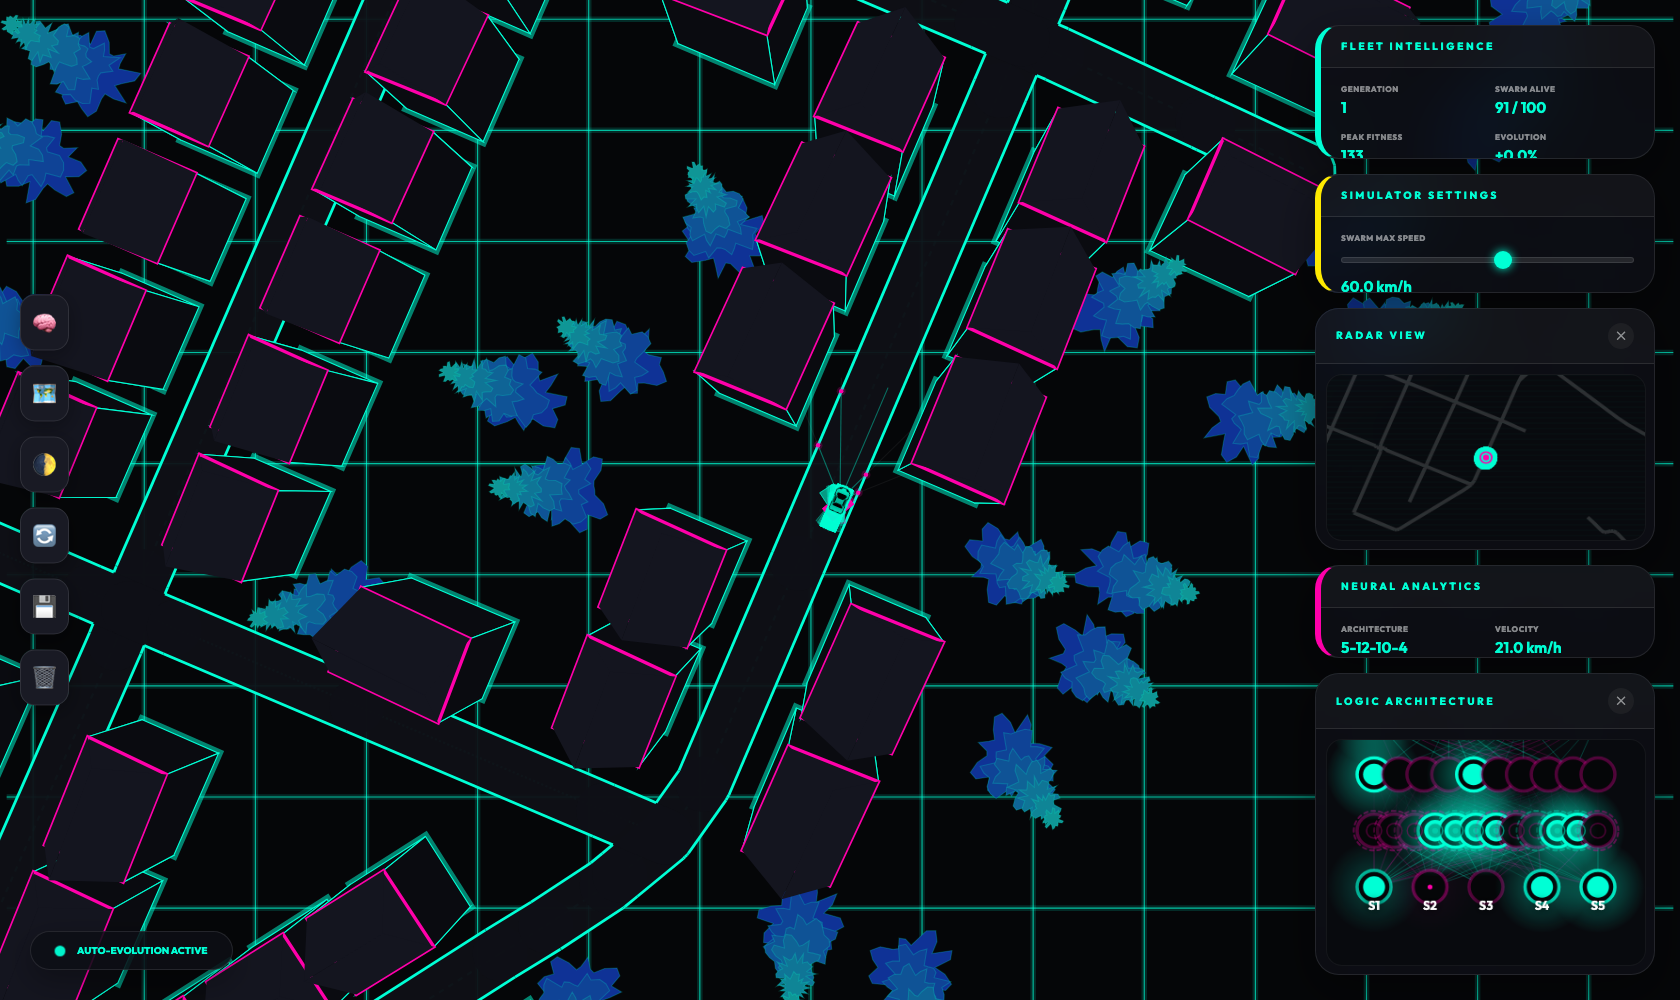
\includegraphics[width=\columnwidth]{figures/sim_early.png}
\caption{The delivered application running, captured unedited from the repaired build. The lead vehicle is drawn with its five LiDAR beams; surviving swarm members are translucent boxes. The right-hand column shows the fleet panel (generation index, survivors, peak fitness, generation-over-generation change), the speed control, the radar minimap, the neural analytics panel and the live network visualiser.}
\label{fig:screenshot}
\end{figure}

Fig.~\ref{fig:neuro} shows the network visualiser in detail. It is the component that best illustrates the transparency argument made in Section~\ref{sec:related}: the five input nodes are labelled with their sensor index, the two hidden layers and the four outputs are drawn with their live activation state, and every connection is drawn with a thickness proportional to how much that weight has changed since the start of the generation. Nothing in the network is hidden behind an abstraction.

The instrumentation panels in the same session read generation 10, six of one hundred individuals still alive, and a peak fitness of 16,384 px against the map's longest reachable route distance of 17,822 px — an independent confirmation, from the interactive build rather than the harness, that the repaired objective produces agents which traverse most of the reachable network. Every metric on those panels nonetheless describes the current best individual or the population size; none describes the dispersion of fitness within the generation, which is exactly the quantity that would have exposed the defect and is the omission analysed in Section~\ref{sec:discussion}.

\begin{figure}[!t]
\centering
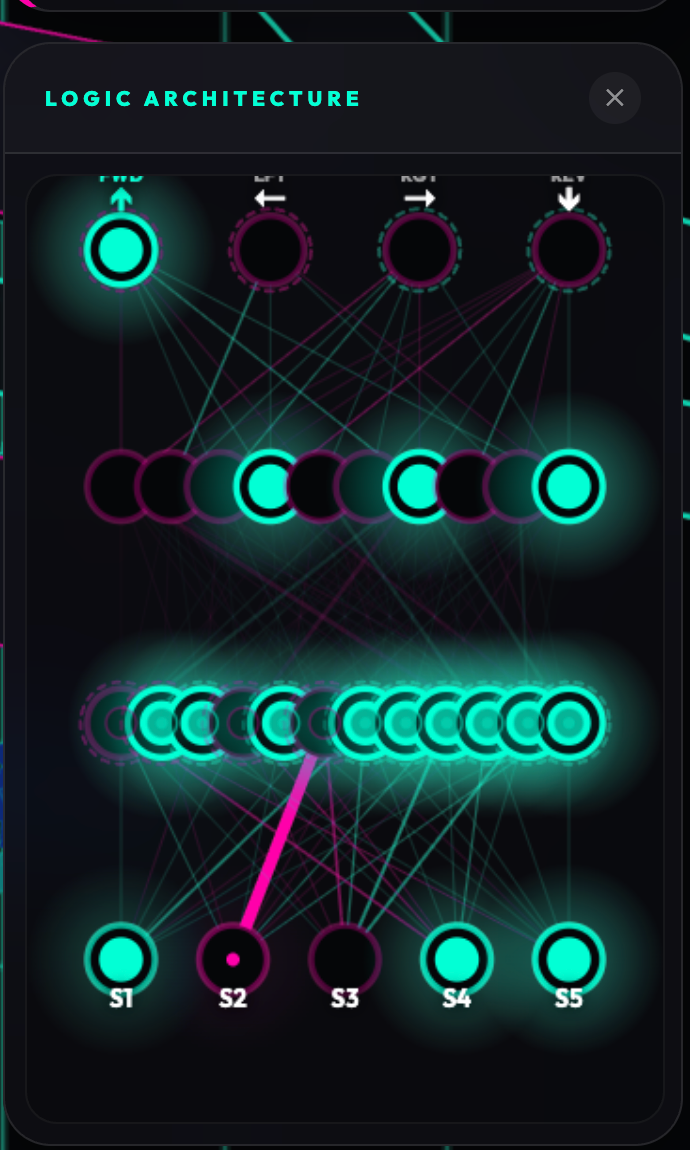
\includegraphics[width=\columnwidth]{figures/neural_panel.png}
\caption{The live network visualiser at the same instant, showing the 5-12-10-4 topology with sensor inputs S1 to S5 at the bottom and the four actuator outputs (forward, left, right, reverse) at the top. Filled nodes are active. Connection thickness encodes how much that weight has changed since the start of the generation rather than its absolute value, so the single heavy magenta edge from sensor S2 is the connection this generation's mutation has moved furthest — here a strongly inhibitory link from the left-of-centre beam.}
\label{fig:neuro}
\end{figure}

\subsection{Computational complexity}

The cost of the pipeline is worth stating explicitly, because it determined the experimental budget. Let n be the number of road-boundary segments, m the number of graph nodes, e the number of graph edges, b the beam count, P the population and G the generations.

\begin{itemize}
\item \textbf{World construction} is dominated by the boolean polygon union, which compares every pair of envelope polygons and splits intersecting edges: O(k²·s²) for k envelopes of s edges each. It runs once, offline, and its output is what is serialised into the map file.
\item \textbf{Dijkstra} over the centreline graph is O((m + e) log m) with a binary heap. The shipped implementation uses a sort-on-insert list, which is O(e·m log m) in the worst case; at m = 446 this is still milliseconds, so it was left as-is in the interactive build and replaced with a heap only in the harness.
\item \textbf{Per-frame sensing} is O(b·n) in the naive form. The interactive engine reduces the effective n by a radius scan, itself O(n) per frame; the harness reduces it to O(b·n\_local) with a uniform grid, where n\_local is typically one to two dozen segments.
\item \textbf{Per-frame inference} is O(Σ w\_i·w\_\{i+1\}) over layer widths — 246 multiply-accumulates for the 5–12–10–4 network, which is negligible beside sensing.
\item \textbf{A training run} is therefore O(P·G·T·(b·n\_local + |θ|)) for an episode horizon T. With P = 60, G = 30 and T ≤ 1,200, a single run completes in tens of seconds, which is what made 20 independent runs plus a 14-variant ablation grid affordable on a laptop.
\end{itemize}

The one place where an asymptotic improvement mattered in practice was sensing. Replacing the linear radius scan with the uniform grid is what moved the full protocol from an overnight job to 27.4 minutes, and it is the reason the study could afford five seeds per arm rather than one.

\section{Learning Method}

\label{sec:method}

\subsection{Genome and initialisation}

The genome is the full set of weights and biases, serialised as nested arrays. Initialisation draws every weight and bias uniformly from [−0.1, 0.1]. This is an unusually small range; it was chosen in the original codebase so that the live network visualisation would render thin connection lines in the first generation. The side effect is that pre-activations start close to zero, so initial outputs are decided almost entirely by the sign of a small random sum. The population is consequently near-degenerate at generation 1, and the mutation operator carries essentially the entire burden of producing behavioural diversity — a fact that turns out to explain the ablation result in Section~\ref{sec:results}.

\subsection{Fitness definitions}

Three fitness definitions are compared, all evaluated at the moment the episode terminates:

\begin{itemize}
\item \textbf{F1 — as-committed route progress.} The score returned by the shipped \texttt{RouteDiscovery} class over the graph as the shipped loader produced it.
\item \textbf{F2 — Euclidean displacement.} Straight-line distance from the start position; the behaviour the codebase falls back to when no route scorer is present.
\item \textbf{F3 — corrected route progress.} The same Dijkstra field, with node identity repaired.
\end{itemize}

Because the termination rules themselves consult the fitness value — an agent whose score has not increased sufficiently is killed for stagnation — changing the fitness definition changes the environment as well as the objective. This coupling is faithful to the real system and is reported as such rather than being factored out; the consequence for experimental design is noted in Section~\ref{sec:limitations}.

\subsection{Termination as implicit reward shaping}

The simulator terminates an episode under five conditions, four of which are hand-written behavioural constraints rather than physical events:

\begin{itemize}
\item collision with a road boundary (physical);
\item fewer than 15 units of fitness gained in any 30-frame window (stagnation);
\item speed below 0.5 for more than 15 consecutive frames (crawling);
\item speed below −0.5 for more than 20 consecutive frames (sustained reversing);
\item four or more sign changes of velocity within a 20-frame window (oscillation).
\end{itemize}

These rules constitute a substantial, undeclared shaping term. They forbid stopping, forbid reversing out of a dead end, and forbid three-point turns — all behaviours a competent driver needs. They were introduced to stop the population converging on degenerate stall-in-place policies, which is a legitimate motivation, but their effect on the achievable policy class is significant and is revisited in Section~\ref{sec:limitations}.

\subsection{Reproduction operators}

The shipped operator, denoted \textbf{clone-elite}, copies the champion genome to the entire next population; index 0 is left unmutated and every other individual is mutated, with every fifth individual receiving an elevated rate. The proposed alternative, \textbf{tournament-crossover}, retains the top 2 genomes unchanged, then fills the population by drawing two parents by tournament of size 3, combining them with uniform crossover over every weight and bias, and mutating the child. Both use the identical mutation kernel taken from the project source, so the comparison isolates selection and recombination rather than confounding them with a new mutation distribution.

That kernel perturbs each parameter independently with probability equal to the mutation rate. A perturbed weight is completely re-randomised in [−2, 2] with probability 0.1 and otherwise receives an additive uniform perturbation in [−0.5, 0.5]; weights are clipped to [−5, 5] and biases to [−2, 2].

\subsection{The training loop in full}

Stated compactly, and with the coupling between fitness and termination made explicit, the training procedure is:

\begin{verbatim}
initialise P genomes ~ U(-0.1, 0.1)
for g = 1 .. G:
    for each genome i:
        v <- fresh vehicle at the start pose
        v.brain <- genome[i]
        while v alive and frames < T:
            borders <- grid.query(v.centre, 400)
            v.update(borders)            # move, score, test
                                         # termination, collide, sense
            s <- 1 - lidar offsets       # 5 features in [0,1]
            a <- threshold(MLP(s))       # 4 bits
            resolve conflicts(a); write to actuators
        fitness[i] <- v.survivalScore    # value at termination
    champion <- argmax fitness
    record best / mean / sd / #distinct(fitness)
    next <- reproduce(genomes, fitness)  # operator under test
    genomes <- next
return best genome seen
\end{verbatim}

Two details in this loop are easy to overlook and both matter. First, the actuator command computed on frame t is applied by the physics on frame t + 1, because sensing happens at the end of \texttt{update}; every controller in the study therefore operates with one frame of delay, and the comparison is unaffected because the delay is identical for all of them. Second, \texttt{v.update} evaluates the termination rules \emph{before} the collision test, so an agent that would have crashed on the same frame it stalls is recorded as a stagnation rather than a collision. This ordering is inherited from the interactive engine and is preserved rather than corrected, but it means the collision and stagnation shares in Fig.~\ref{fig:termination} should be read as a partition under that convention rather than as independent event rates.

\subsection{Hyperparameters}

The full configuration is listed in Table~\ref{tab:hyper}. Population size was reduced from the interactive system's 100 to 60 in order to fit 20 independent training runs plus the ablation grid into the available compute budget; the reduction applies uniformly to every arm, so the comparison between arms is unaffected, though absolute performance is a lower bound on what a longer budget would reach.

\begin{table}[!t]
\caption{Experimental configuration}
\label{tab:hyper}
\centering
\footnotesize
\begin{tabular}{lr}
\toprule
Parameter & Value \\
\midrule
\multicolumn{2}{l}{\emph{Evolution}} \\
Population size & 60 \\
Generations (main runs) & 30 \\
Generations (ablations) & 20 \\
Independent seeds (main) & 11, 22, 33, 44, 55 \\
Independent seeds (ablations) & 3 \\
Elite count (tournament arm) & 2 \\
Tournament size & 3 \\
Mutation rate & 0.15 \\
Elevated rate, every 5th individual & 0.50 \\
\multicolumn{2}{l}{\emph{Network}} \\
Layer widths & 5 – 12 – 10 – 4 \\
Trainable parameters & 246 \\
Activation & logistic, thresholded at 0.5 \\
Weight and bias initialisation & U(−0.1, 0.1) \\
\multicolumn{2}{l}{\emph{Vehicle and sensing}} \\
Beams / field of view / range & 5 / π/2 / 220 px \\
Vehicle size & 30 × 50 px \\
Max speed / acceleration / friction & 6 / 0.2 / 0.05 \\
Steering increment & 0.07 rad per frame \\
\multicolumn{2}{l}{\emph{Episodes and evaluation}} \\
Frame budget & 1,200 (20 s at 60 fps) \\
Validation / test poses & 10 / 20 \\
Bootstrap resamples & 2,000 \\
Master seed & 2026 \\
\bottomrule
\end{tabular}
\end{table}

\section{Baselines}

\label{sec:baselines}

Four reference controllers are implemented. All four consume the identical five-element observation vector and write the identical four actuator bits, so any performance difference is attributable to the policy rather than to a sensing or actuation advantage — with the single, deliberate exception of the oracle.

\subsection{B0 — Random network}

An untrained multilayer perceptron drawn from the project's own initialiser. This is the floor: any method that does not beat it has learned nothing. Because it is stochastic it is evaluated across all 5 seeds at every pose.

\subsection{B1 — Reactive finite-state heuristic}

The rule-based controller promised in the Milestone 1 definition. It drives forward unconditionally; if the centre beam reports an obstacle beyond a block threshold, or the summed left and right readings differ by more than an asymmetry threshold, it steers toward the freer side; if the centre beam exceeds a brake threshold it lifts the throttle. Three parameters, grid-searched on the validation poses.

\subsection{B2 — Proportional steering controller}

The geometric "PID-style" controller from the Milestone 1 definition, reduced to its proportional term because the plant has no integrator worth winding up over a twenty-second episode and the actuator is binary. A signed error is formed by weighting each beam by its lateral position and summing:

\begin{equation}
u = \frac{k_p}{n}\sum_{i=1}^{n} -\,\frac{i - (n-1)/2}{(n-1)/2}\; s_i
\end{equation}

and discretised through a dead-band: steer left if u exceeds the dead-band, right if it falls below its negative, straight otherwise. The quantisation is a genuine handicap and is acknowledged as such — a continuous-steering plant would suit this controller considerably better, and its relative weakness in Table~\ref{tab:final} should be read in that light.

\subsection{B3 — Pure-pursuit reference (oracle)}

A path-tracking controller in the sense of Coulter \cite{coulter}, given privileged access to the road centreline graph and the route-distance field. It selects the point on a nearby centreline whose route distance exceeds the vehicle's current progress by a look-ahead distance, restricted to the forward half-plane, and steers toward it. The forward restriction is necessary precisely because the distance field is radial: without it, the controller periodically selects an equidistant point on a branch behind the vehicle and turns around — a failure that itself illustrates the objective's ambiguity.

This controller is \textbf{not a competitor}. It observes information the learned agents never see. It is included to answer a question the learned-versus-heuristic comparison cannot: how much of the residual failure rate is attributable to the policy, and how much to the actuator resolution and road geometry that constrain every policy equally.

\subsection{Baseline tuning protocol}

Each hand-written controller was grid-searched on the 10 validation poses. The searches covered 45 configurations for the reactive heuristic, 72 for the proportional controller and 6 look-ahead distances for pure pursuit. The selected settings are listed in Table~\ref{tab:tuning}. This step matters: an untuned proportional controller scored well under half of its tuned counterpart in preliminary runs, and reporting the untuned number would have manufactured an advantage for the learned agent.

\begin{table}[!t]
\caption{Baseline hyperparameters selected on validation poses}
\label{tab:tuning}
\centering
\footnotesize
\begin{tabular}{lrrr}
\toprule
Controller & Grid & Selected & Val. route (px) \\
\midrule
Reactive FSM & 45 & block 0.35, brake 0.75, asym. 0.25 & 4,721 \\
P-controller & 72 & kp 0.8, dead-band 0.15, brake 0.95 & 938 \\
Pure pursuit (oracle) & 6 & look-ahead 120 px & 1,909 \\
\bottomrule
\end{tabular}
\\[2pt]\parbox{\linewidth}{\scriptsize Full grids are recorded in \texttt{experiments/results/e2a\_baseline\_tuning.json}.}
\end{table}

The sensitivity of each baseline to its own parameters is itself informative, and is reported in Table~\ref{tab:sensitivity} so that a reader can judge how much the selection depended on the particular validation poses. The reactive heuristic spans a factor of 1.5 between its best and worst configuration, and the proportional controller a factor of 15.5. Neither best configuration sits on the edge of its grid on every axis, which is weak evidence that the searches were wide enough.

\begin{table*}[!t]
\caption{Baseline tuning sensitivity: best and worst configurations}
\label{tab:sensitivity}
\centering
\footnotesize
\begin{tabular}{lrrr}
\toprule
Controller & Rank & Configuration & Val. route (px) \\
\midrule
\multicolumn{4}{l}{\emph{Reactive FSM}} \\
 & best & blockThreshold=0.35, brakeThreshold=0.75, asymmetry=0.25 & 4,721 \\
 & 2nd & blockThreshold=0.35, brakeThreshold=0.85, asymmetry=0.25 & 4,721 \\
 & 3rd & blockThreshold=0.35, brakeThreshold=0.95, asymmetry=0.25 & 4,721 \\
 & median & blockThreshold=0.65, brakeThreshold=0.95, asymmetry=0.1 & 3,834 \\
 & worst & blockThreshold=0.35, brakeThreshold=0.95, asymmetry=0.1 & 3,171 \\
\multicolumn{4}{l}{\emph{P-controller}} \\
 & best & kp=0.8, deadband=0.15, brakeThreshold=0.95 & 938 \\
 & 2nd & kp=0.8, deadband=0.15, brakeThreshold=0.85 & 938 \\
 & 3rd & kp=0.8, deadband=0.15, brakeThreshold=0.75 & 938 \\
 & median & kp=2.2, deadband=0.05, brakeThreshold=0.95 & 142 \\
 & worst & kp=8, deadband=0.02, brakeThreshold=0.75 & 60 \\
\multicolumn{4}{l}{\emph{Pure pursuit (oracle)}} \\
 & best & lookahead=120 & 1,909 \\
 & 2nd & lookahead=180 & 1,337 \\
 & 3rd & lookahead=220 & 1,052 \\
 & median & lookahead=300 & 851 \\
 & worst & lookahead=550 & 627 \\
\bottomrule
\end{tabular}
\\[2pt]\parbox{\linewidth}{\scriptsize Configurations are ranked by mean route progress over the validation poses. Only the best row of each group is used in any reported comparison.}
\end{table*}

\section{Experimental Protocol}

\label{sec:protocol}

\subsection{Metrics}

Nine per-episode metrics are recorded. The primary outcome is \textbf{peak route progress}: the maximum route-distance value attained during the episode, measured with the corrected scorer \emph{regardless of which fitness the agent was trained on}. Keeping the measurement independent of the training signal is what makes the arms comparable at all — an arm trained on a broken objective must still be scored on a working one.

\begin{itemize}
\item \textbf{Peak route progress (px)} — primary outcome; distance along the road network from the start.
\item \textbf{Frames survived} — episode length at 60 fps.
\item \textbf{Collision rate} — share of episodes ending in boundary contact.
\item \textbf{Termination mix} — collision, stagnation or reversal, or survival to the frame budget.
\item \textbf{Path length (px)} — integrated speed, i.e. distance actually driven.
\item \textbf{Mean distance between failures (MDBF)} — total path length divided by collision count.
\item \textbf{RMS jerk} — root-mean-square second difference of speed; a comfort proxy.
\item \textbf{Steering reversals per 1000 frames} — a smoothness proxy for control chatter.
\item \textbf{Mean lateral deviation and off-corridor share} — distance from the nearest centreline, and the fraction of frames spent more than a road half-width away from it.
\end{itemize}

\subsection{Statistical methodology}

The distributions involved are bounded below, heavy-tailed and frequently bimodal — an agent either threads a junction or dies at it — so Gaussian assumptions are avoided throughout. The unit of analysis for the headline comparison is the \textbf{pose mean}: for each arm and each test pose, the metric is averaged over seeds, yielding one value per pose. This pairs the arms on identical initial conditions and prevents an arm with more seeds from acquiring spurious precision.

\begin{itemize}
\item Central tendency and dispersion are reported as mean, standard deviation, median and quartiles.
\item Confidence intervals on the mean are percentile bootstrap intervals \cite{efron} with 2,000 resamples, drawn from a seeded generator so the intervals are themselves reproducible.
\item Location differences are tested with the Mann–Whitney U test \cite{mannwhitney} using the tie-corrected normal approximation.
\item Effect sizes are reported as Cliff's delta \cite{cliff}, with the conventional thresholds 0.147, 0.33 and 0.474 for small, medium and large.
\end{itemize}

No correction for multiple comparisons is applied, and the tests should be read as descriptive rather than confirmatory: with 20 paired poses the power to detect anything but a large effect is limited. Saying so is more useful than presenting borderline p-values as though they settled the question.

\subsection{Compute budget and determinism}

The full protocol ran in 27.4 minutes on Apple M5 (10 logical cores, 16 GB RAM) under Node.js v24.16.0, single-threaded and CPU-only. No GPU is used anywhere in this project, because the models are hand-written and gradient-free. Approximately 86,400 episodes were simulated in total. Every stochastic component draws from a seeded mulberry32 generator installed in place of \texttt{Math.random} inside the simulation context, so a given seed reproduces a run exactly.

\subsection{Experiment matrix}

\begin{itemize}
\item \textbf{E1 — Fitness-signal diagnostic.} One generation of random genomes evaluated under each of the three fitness definitions, measuring how many distinct fitness values the objective actually produces.
\item \textbf{E2 — Fixed-policy baselines.} All four reference controllers on validation and test poses, after tuning.
\item \textbf{E3 — Training arms.} Four arms × 5 seeds × 30 generations × 60 individuals.
\item \textbf{E4 — Ablations.} 14 variants over architecture, mutation rate, beam count and beam range, 3 seeds each, selected on validation poses only.
\item \textbf{E5 — Held-out evaluation.} Every champion and every tuned baseline on the test poses, used exactly once.
\end{itemize}

\section{Results}

\label{sec:results}

\subsection{E1: the committed objective carries no selection signal}

The route-progress scorer keys its adjacency and distance maps on a node identifier, \texttt{GeoPoint.id}. The graph loader reconstructs every node with \texttt{new GeoPoint(x, y)}, and that constructor assigns only the two coordinates. Every identifier is therefore \texttt{undefined}, all 446 nodes collapse onto a single map entry, the relaxation loop never fires, and the interpolation in the scorer evaluates to zero everywhere in the world.

The consequences are measured directly. Across a population of 60 randomly initialised networks evaluated from the training pose, the as-committed objective produced \textbf{1 distinct fitness value} — every individual scored identically — against 26 for Euclidean displacement and 27 for the corrected scorer (Fig.~\ref{fig:signal}). Selection over a constant objective is selection at random.

The damage is not confined to selection. Because the stagnation rule requires the fitness value to increase by at least 15 units every 30 frames, a constant fitness of zero guarantees the rule fires as soon as it has enough history. Mean episode length collapses from 84.2 frames under the corrected objective to 39.1 frames — roughly 0.7 seconds — under the committed one (Fig.~\ref{fig:signalframes}). Agents were being executed for barely a second before being destroyed for failing to make progress on a metric that could not move.

\begin{figure*}[!t]
\centering

\includegraphics[width=\textwidth]{figures/fig_signal}
\caption{Selection signal available to the genetic algorithm. The as-committed objective yields a single distinct fitness value across the whole population, so the champion is chosen arbitrarily.}
\label{fig:signal}
\end{figure*}

\begin{figure*}[!t]
\centering

\includegraphics[width=\textwidth]{figures/fig_signal_frames}
\caption{Mean episode length under each objective. The degenerate objective interacts with the stagnation rule to terminate agents almost immediately, compounding the loss of selection pressure with a loss of experience.}
\label{fig:signalframes}
\end{figure*}

\begin{table}[!t]
\caption{Fitness-signal diagnostic (E1)}
\label{tab:signal}
\centering
\footnotesize
\begin{tabular}{lrrrr}
\toprule
Objective & Distinct fitness & Mean fitness & Mean frames & Route reached (px) \\
\midrule
as-committed (RouteDiscovery) & 1 / 60 & 0.0 & 39.1 & 230 \\
euclidean fallback & 26 / 60 & 370.7 & 84.8 & 651 \\
corrected route scorer & 27 / 60 & 613.4 & 84.2 & 651 \\
\bottomrule
\end{tabular}
\\[2pt]\parbox{\linewidth}{\scriptsize Randomly initialised networks, identical seeds across rows. Route reached is measured with the corrected scorer in every row, so the last column is comparable even though the fitness column is not.}
\end{table}

The defect is a contract mismatch between two modules that are individually reasonable. The loader is not wrong to construct a point from coordinates; the scorer is not wrong to key on an identifier that the serialised map file genuinely contains. The fault lies in the undeclared dependency between them — exactly the category Sculley et al. describe as an undeclared consumer \cite{sculley}. It produces no exception, no warning and no visible change in the simulation.

\begin{quote}\small\textbf{Repair.} Two changes were made to the live code. \texttt{NodeGraph.load} now preserves the OpenStreetMap node identifier and the one-way tag rather than discarding them, and \texttt{RouteDiscovery} now keys its maps on node index, which is always well defined regardless of what the loader supplies. After the repair the distance map contains one entry per node, 428 of 446 nodes are reachable, and the field spans 0 to 17,822 px. The baseline arm in every experiment below uses a pinned verbatim copy of both the pre-repair scorer and the pre-repair loader, so the comparison remains valid against the repaired working tree.\end{quote}

\subsection{E3: what each objective and operator actually learns}

Fig.~\ref{fig:learning} shows learning curves for the four training arms and Table~\ref{tab:training} summarises them. The as-committed arm is a flat line: best fitness is 0.0 ± 0.0 across all 5 seeds, and the mean number of distinct fitness values per generation is 1.0 — that is, exactly one, in every generation of every seed. The route progress its champions happen to achieve, 284 px, is identical at generation 30 to what it was at generation 1 (284 px). Thirty generations of evolution produced no improvement whatsoever, which is the expected outcome of optimising a constant.

Repairing the objective changes this completely. The corrected route arm reaches 6,500 ± 5,604 best fitness with 34.9 distinct fitness values per generation, and the Euclidean arm reaches 3,542 ± 1,311. Both are learning. The difference between them is instructive: Euclidean displacement rewards getting geometrically far from the origin, which on a road network is best achieved by heading across the map in a straight line, whereas route progress rewards distance \emph{along the roads}. The route objective therefore produces higher route scores by construction, but it also produces higher variance, because a policy that commits to a long branch is rewarded far more than one that circles near the origin.

The two reproduction operators separate on variance rather than on peak. Clone-elite reaches a mean best fitness of 6,500 with a standard deviation of 5,604 across seeds; tournament with uniform crossover reaches 5,920 with a standard deviation of 1,690 — a 3.3× reduction in seed-to-seed spread. Its final-generation champions also travel further (9,607 px against 6,500 px). The interpretation is that cloning the champion into the entire population destroys diversity every generation, so the run's outcome is decided by whichever lineage happens to be lucky early; maintaining a population and recombining it makes the search less dependent on that accident.

\begin{figure*}[!t]
\centering

\includegraphics[width=\textwidth]{figures/fig_learning}
\caption{Learning curves: best route progress reached by the champion of each generation, averaged over seeds, with the band spanning the minimum and maximum across seeds. The as-committed arm is flat by construction.}
\label{fig:learning}
\end{figure*}

\begin{figure*}[!t]
\centering

\includegraphics[width=\textwidth]{figures/fig_selection}
\caption{Distinct fitness values per generation. This is the quantity that determines whether selection can act at all; the as-committed arm sits at exactly one for the entire run, in every seed.}
\label{fig:selection}
\end{figure*}

\begin{table}[!t]
\caption{Training arms (E3): mean ± SD over seeds}
\label{tab:training}
\centering
\footnotesize
\begin{tabular}{lrrrr}
\toprule
Arm & Best fitness & Final route (px) & Distinct fit./gen & Wall (s) \\
\midrule
NE-A as-committed & 0 ± 0 & 284 ± 227 & 1.0 & 18 \\
NE-B Euclidean & 3,542 ± 1,311 & 4,888 ± 1,595 & 31.9 & 30 \\
NE-C route & 6,500 ± 5,604 & 6,500 ± 5,604 & 34.9 & 34 \\
NE-D route + crossover & 5,920 ± 1,690 & 9,607 ± 6,289 & 28.2 & 42 \\
\bottomrule
\end{tabular}
\\[2pt]\parbox{\linewidth}{\scriptsize 5 seeds per arm, 60 individuals, 30 generations. Fitness is on each arm's own scale and is comparable only within an arm; route progress is measured with the corrected scorer for all arms and is comparable across rows.}
\end{table}

Table~\ref{tab:curve} gives the same information numerically at five-generation intervals, which makes two features visible that the plot smooths over. The first is that most of the improvement in the working arms happens early: by generation 10 the corrected arms have reached a large fraction of their final value, and the remaining twenty generations add comparatively little. The second is that the number of distinct fitness values does not decay toward one in the tournament arm the way it does under clone-elite, which is the mechanism behind the variance reduction reported above.

\begin{table*}[!t]
\caption{Learning curves at five-generation intervals (mean over seeds)}
\label{tab:curve}
\centering
\footnotesize
\begin{tabular}{lrrrrrr}
\toprule
Gen & NE-A & NE-B & NE-C & NE-D & NE-C dist. & NE-D dist. \\
\midrule
1 & 284 & 3,421 & 3,629 & 3,629 & 33.4 & 33.4 \\
5 & 284 & 3,871 & 3,746 & 3,755 & 31.2 & 30.6 \\
10 & 284 & 4,165 & 6,138 & 3,761 & 30.6 & 28.2 \\
15 & 284 & 4,776 & 6,132 & 4,897 & 36.0 & 29.8 \\
20 & 284 & 4,802 & 6,385 & 7,296 & 34.8 & 28.0 \\
25 & 284 & 4,877 & 6,404 & 9,607 & 38.8 & 25.4 \\
30 & 284 & 4,888 & 6,500 & 9,607 & 37.4 & 23.8 \\
\bottomrule
\end{tabular}
\\[2pt]\parbox{\linewidth}{\scriptsize Route progress of the generation champion in pixels, and the number of distinct fitness values in that generation, both averaged over seeds. The as-committed arm's distinct-fitness count is 1 at every generation of every seed and is omitted for space.}
\end{table*}

\subsection{Why higher training fitness did not mean better transfer}

The clone-elite arm reached the higher training-condition fitness (6,500 against 5,920) yet the lower held-out score (841 px against 2,646 px). That inversion is the clearest evidence of overfitting in the study, and it has a specific mechanism rather than a generic one.

Under clone-elite, the entire next population is a mutated copy of one genome. Diversity is destroyed and regenerated every generation from a single point, so the search behaves like a stochastic hill-climb from whichever lineage first found a long branch out of the training pose. A policy that has specialised to the exact sequence of turns leaving that one start will score extremely well there — the best single run in the study reached 16,433 — and will have no reason to generalise. Tournament selection with crossover keeps several lineages alive and recombines them, which both caps how far any one of them can specialise and preserves behavioural variation that happens to be useful elsewhere.

The practical implication for anyone extending this work is that training-condition fitness is not a model-selection criterion here. Every ablation in Section~\ref{sec:results} is therefore selected on validation poses rather than on training fitness, and Table~\ref{tab:ablation} reports both so that the divergence between them can be seen directly.

\subsection{E5: held-out comparison}

Table~\ref{tab:final} and Fig.~\ref{fig:final} give the headline result on the 20 test poses. The strongest learned arm, NE-D route + crossover, reaches 2,646 px of route progress (bootstrap 95\% CI 2,053–3,278 px), against 4,793 px for the tuned reactive heuristic, 908 px for the tuned proportional controller and 2,312 px for the map-privileged pure-pursuit reference.

Against the reactive heuristic the comparison favours the hand-written heuristic: Mann–Whitney U = 97, z = -2.79, p = 0.005, Cliff's delta = -0.52 (large). Against the as-committed arm the separation is p = 0.000 with Cliff's delta = 0.91 (large), confirming that repairing the objective produces a difference that survives a non-parametric test on held-out conditions and is not an artefact of the training curve.

\begin{figure*}[!t]
\centering

\includegraphics[width=\textwidth]{figures/fig_final}
\caption{Route progress on held-out start poses, ranked. Whiskers are percentile bootstrap 95\% confidence intervals on the mean of per-pose means. The oracle is drawn in grey because it observes the map and is a ceiling rather than a competitor.}
\label{fig:final}
\end{figure*}

\begin{table*}[!t]
\caption{Held-out evaluation (E5), ranked by route progress}
\label{tab:final}
\centering
\footnotesize
\begin{tabular}{lrrrrr}
\toprule
Controller & Route (px) & 95\% CI & Collision & Frames & MDBF (px) \\
\midrule
Reactive FSM & 4,793 & 3,654–6,131 & 80\% & 580 & 4,159 \\
NE-D route + crossover & 2,646 & 2,053–3,278 & 80\% & 408 & 2,864 \\
Pure pursuit (oracle) & 2,312 & 1,594–3,080 & 85\% & 353 & 2,330 \\
NE-B Euclidean & 1,428 & 1,082–1,784 & 78\% & 221 & 1,537 \\
P-controller & 908 & 480–1,454 & 100\% & 169 & 889 \\
NE-C route & 841 & 643–1,064 & 98\% & 157 & 828 \\
NE-A as-committed & 404 & 225–626 & 33\% & 87 & 1,185 \\
\bottomrule
\end{tabular}
\\[2pt]\parbox{\linewidth}{\scriptsize 20 held-out poses; learned arms additionally averaged over 5 seeds. MDBF is total distance driven per collision. The oracle observes the road graph and is a reference, not a competing method.}
\end{table*}

Table~\ref{tab:tests} reports every pairwise comparison against the strongest learned arm. The pattern is that the large, unambiguous separations are against the degenerate arm and against the weakest hand-written controller, while the comparisons among the credible controllers are not resolved at 20 paired poses. That is an honest reading of the evidence: this study can establish that repairing the objective mattered, and cannot establish a reliable ordering among the controllers that work.

\begin{table*}[!t]
\caption{Pairwise comparisons against the strongest learned arm}
\label{tab:tests}
\centering
\footnotesize
\begin{tabular}{lrrrrrrr}
\toprule
Comparison & Mean A & Mean B & U & z & p & Cliff's d & Magnitude \\
\midrule
NE-D vs NE-A as-committed & 2,646 & 404 & 19 & 4.90 & 0.000 & 0.91 & large \\
NE-D vs NE-B Euclidean & 2,646 & 1,428 & 96 & 2.81 & 0.005 & 0.52 & large \\
NE-D vs NE-C route & 2,646 & 841 & 58 & 3.84 & 0.000 & 0.71 & large \\
NE-D vs Reactive FSM & 2,646 & 4,793 & 97 & -2.79 & 0.005 & -0.52 & large \\
NE-D vs P-controller & 2,646 & 908 & 61 & 3.76 & 0.000 & 0.69 & large \\
NE-D vs Pure pursuit (oracle) & 2,646 & 2,312 & 169 & 0.84 & 0.402 & 0.15 & small \\
\bottomrule
\end{tabular}
\\[2pt]\parbox{\linewidth}{\scriptsize Mann–Whitney U on per-pose means of peak route progress, tie-corrected normal approximation, two-sided. A positive Cliff's delta favours NE-D. No multiple-comparison correction is applied; see the caveat in Section VIII.}
\end{table*}

\subsection{Per-pose behaviour and the generalisation gap}

Averages conceal the shape of the distribution, which in this task is strongly bimodal. Table~\ref{tab:perpose} gives the per-pose means for the four most informative controllers on every test pose. The pattern is consistent: on a handful of poses several controllers travel thousands of pixels, and on the remainder every controller fails within a few hundred. Those poses are not random — they are the ones whose first junction lies within the vehicle's stopping distance of the start.

\begin{table*}[!t]
\caption{Per-pose route progress (px) on the held-out test set}
\label{tab:perpose}
\centering
\footnotesize
\begin{tabular}{lrrrr}
\toprule
Pose & NE-D & NE-C & Reactive FSM & Pure pursuit \\
\midrule
P10 & 1,692 & 694 & 2,824 & 1,901 \\
P11 & 446 & 323 & 1,538 & 874 \\
P12 & 2,437 & 1,461 & 3,530 & 1,072 \\
P13 & 3,694 & 270 & 6,830 & 846 \\
P14 & 742 & 274 & 3,406 & 1,198 \\
P15 & 4,561 & 786 & 6,999 & 3,235 \\
P16 & 3,519 & 1,757 & 5,492 & 4,886 \\
P17 & 509 & 17 & 2,967 & 668 \\
P18 & 4,524 & 1,179 & 5,569 & 3,188 \\
P19 & 4,467 & 770 & 7,243 & 7,177 \\
P20 & 2,138 & 739 & 3,843 & 1,828 \\
P21 & 1,627 & 869 & 3,111 & 535 \\
P22 & 3,392 & 1,250 & 4,744 & 39 \\
P23 & 1,195 & 880 & 1,213 & 3,349 \\
P24 & 4,797 & 821 & 14,611 & 1,615 \\
P25 & 3,545 & 1,834 & 7,334 & 1,932 \\
P26 & 3,131 & 769 & 3,761 & 3,761 \\
P27 & 2,920 & 985 & 5,000 & 2,950 \\
P28 & 979 & 602 & 2,050 & 1,375 \\
P29 & 2,597 & 546 & 3,805 & 3,805 \\
\bottomrule
\end{tabular}
\\[2pt]\parbox{\linewidth}{\scriptsize Each cell is the mean over seeds for that arm at that pose. The learned arms are averaged over five seeds; the hand-written controllers are deterministic given a pose.}
\end{table*}

The baselines provide an independent check on whether the pose split is fair. Because the hand-written controllers were tuned on the validation poses and then evaluated on the test poses, the difference between their validation and test scores measures how much the tuning over-fitted the validation set. Table~\ref{tab:gengap} reports it. The reactive heuristic transfers at 4,793 px against 4,721 px on validation, and the pure-pursuit reference at 2,312 px against 1,909 px. Neither shows the collapse that would indicate a badly split or unrepresentative test set.

\begin{table}[!t]
\caption{Validation-to-test transfer of the fixed policies}
\label{tab:gengap}
\centering
\footnotesize
\begin{tabular}{lrrrr}
\toprule
Controller & Val. route (px) & Test route (px) & Val. coll. & Test coll. \\
\midrule
Random NN & 217 & 311 & 20\% & 26\% \\
Reactive FSM & 4,721 & 4,793 & 60\% & 80\% \\
P-controller & 938 & 908 & 100\% & 100\% \\
Pure pursuit (oracle) & 1,909 & 2,312 & 80\% & 85\% \\
\bottomrule
\end{tabular}
\\[2pt]\parbox{\linewidth}{\scriptsize The random network is included as the performance floor; every other controller must beat it to have demonstrated anything.}
\end{table}

\subsection{Failure modes}

Fig.~\ref{fig:termination} decomposes how episodes end. The distinction between collision and stagnation is diagnostically important: a collision means the policy drove into a wall, whereas a stagnation termination means the policy stopped making progress and was killed by the behavioural rules — typically by getting stuck against a boundary, oscillating, or entering a dead end it is forbidden to reverse out of.

The single most consequential number in the whole study is the collision rate of the oracle: 85\% of pure-pursuit episodes end in contact with a boundary, despite the controller knowing exactly where the road goes. That is not a defect in the controller; it is a property of the plant. With a steering increment fixed at 0.07 rad per frame and a speed that must stay above 0.5 to avoid the crawling termination, the minimum achievable turning radius is bounded below, and several junctions in this 100 px-wide network simply cannot be negotiated at speed. The residual failure rate common to all controllers is therefore attributable to the vehicle model rather than to the policy, and no amount of additional training will remove it.

\begin{figure*}[!t]
\centering

\includegraphics[width=\textwidth]{figures/fig_termination}
\caption{Termination cause by controller. Survival to the frame budget is the only outcome representing success; stagnation and reversal terminations reflect the behavioural rules described in Section VI.}
\label{fig:termination}
\end{figure*}

\begin{figure*}[!t]
\centering

\includegraphics[width=\textwidth]{figures/fig_traj}
\caption{Single-episode trajectories from the held-out pose at which the two controllers disagree most. From an identical start, the tuned reactive heuristic circles a block and is terminated by the stagnation rule, while the evolved champion continues along the corridor and survives to the frame budget. Both traces are one seed, so the distances shown are individual episodes rather than the seed-averaged pose means reported in Table X.}
\label{fig:traj}
\end{figure*}

\subsection{Comfort and control quality}

Route progress alone does not distinguish a controller that drives smoothly from one that reaches the same place by sawing at the wheel. Table~\ref{tab:comfort} reports RMS jerk, steering reversal rate, mean lateral deviation from the centreline, and the share of frames spent outside the road corridor. These are the smoothness metrics the Milestone 1 definition committed to reporting.

\begin{table*}[!t]
\caption{Control quality on held-out poses}
\label{tab:comfort}
\centering
\footnotesize
\begin{tabular}{lrrrr}
\toprule
Controller & RMS jerk & Steer rev./1k & Lateral dev. (px) & Off-corridor \\
\midrule
Reactive FSM & 0.006 & 41 & 5 & 0\% \\
NE-D route + crossover & 0.010 & 162 & 9 & 0\% \\
Pure pursuit (oracle) & 0.006 & 284 & 6 & 0\% \\
NE-B Euclidean & 0.009 & 146 & 7 & 0\% \\
P-controller & 0.008 & 0 & 8 & 0\% \\
NE-C route & 0.013 & 92 & 8 & 0\% \\
NE-A as-committed & 0.024 & 0 & 4 & 0\% \\
\bottomrule
\end{tabular}
\\[2pt]\parbox{\linewidth}{\scriptsize RMS jerk is the root-mean-square second difference of speed. Off-corridor is the share of frames spent more than one road half-width from the nearest centreline.}
\end{table*}

Two entries deserve comment. The off-corridor share is zero for every controller, which looks like a broken metric and is in fact a structural property of this environment: the road is 100 px wide and its boundary is the collision surface, so a vehicle that leaves the corridor has already ended its episode. The metric can only ever be non-zero in a world where leaving the road is survivable, and it is reported here for completeness rather than because it discriminates.

The steering-reversal column is more informative. The proportional controller records zero reversals, because its tuned dead-band of 0.15 suppresses almost all steering commands — it drives essentially straight until it hits something, which is consistent with its 100\% collision rate. At the other extreme the pure-pursuit reference records 284 reversals per thousand frames: it is continuously correcting toward a look-ahead point it can only approach through a binary actuator, which is precisely the quantisation penalty described in Section~\ref{sec:baselines}. The evolved champion sits between them at 162, and the tuned heuristic is the smoothest of the competitive controllers at 41.

\subsection{E4: ablations}

Table~\ref{tab:ablation} and Fig.~\ref{fig:ablarch} to Fig.~\ref{fig:ablsense} report 14 variants, each trained for 20 generations across 3 seeds and scored on the validation poses. Three findings stand out.

\textbf{Depth hurts.} The best architecture is \emph{no hidden layer [5-4]} at 2,949 px, against 1,358 px for the current 5–12–10–4 network — despite the latter carrying 246 parameters to the former's 24. The Milestone 2 checkpoint listed "expanding the hidden layer depth for improved generalisation" as a next step; the measurement says the opposite. The explanation is the thresholded activation: each unit emits a single bit, so a hidden layer of width w passes at most w bits forward regardless of how many weights feed it, and stacking such layers mostly adds search dimensions without adding expressible behaviour. A five-input, four-output threshold network is close to the point where additional depth is pure cost.

\textbf{Mutation rate is the dominant evolutionary hyperparameter.} The best setting is \emph{rate 0.50} at 1,545 px; across the swept range the validation score varies by a factor of 2.8. Given that the initialisation range is only [−0.1, 0.1], the mutation operator is effectively responsible for the entire exploration budget, so this sensitivity is unsurprising in hindsight — but it was not anticipated, and the shipped value is not the best one tested.

\textbf{Sensing changes less than expected.} The best sensing variant is \emph{7 beams} at 1,790 px, and the spread across sensing variants is a factor of 10.7. Beam count and beam range both move the result, but not as much as the mutation rate does, which suggests the bottleneck in this system is the optimiser and the actuator rather than the perception.

\begin{table*}[!t]
\caption{Ablation study (E4), selected on validation poses}
\label{tab:ablation}
\centering
\footnotesize
\begin{tabular}{lrrr}
\toprule
Variant & Params & Train fitness & Val. route (px) \\
\midrule
\multicolumn{4}{l}{\emph{Architecture}} \\
no hidden layer [5-4] & 24 & 10,015 ± 5,526 & 2,949 ± 277 \\
checkpoint [5-6-4] & 64 & 3,925 ± 606 & 729 ± 200 \\
current [5-12-10-4] & 246 & 5,524 ± 1,357 & 1,358 ± 602 \\
wide [5-24-16-4] & 612 & 4,095 ± 895 & 415 ± 281 \\
\multicolumn{4}{l}{\emph{Mutation}} \\
rate 0.05 & 246 & 4,093 ± 673 & 1,014 ± 183 \\
rate 0.15 (default) & 246 & 5,524 ± 1,357 & 1,358 ± 602 \\
rate 0.30 & 246 & 3,689 ± 191 & 548 ± 322 \\
rate 0.50 & 246 & 4,791 ± 1,964 & 1,545 ± 1,660 \\
\multicolumn{4}{l}{\emph{Sensing}} \\
3 beams & 222 & 3,569 ± 3 & 536 ± 294 \\
5 beams (default) & 246 & 5,524 ± 1,357 & 1,358 ± 602 \\
7 beams & 270 & 6,252 ± 1,515 & 1,790 ± 896 \\
range 120 px & 246 & 3,578 ± 0 & 168 ± 99 \\
range 220 px (default) & 246 & 5,524 ± 1,357 & 1,358 ± 602 \\
range 320 px & 246 & 4,217 ± 1,105 & 935 ± 386 \\
\bottomrule
\end{tabular}
\\[2pt]\parbox{\linewidth}{\scriptsize 3 seeds per variant, 20 generations, tournament-crossover operator with the corrected objective throughout. Test poses were not used at any point in this table.}
\end{table*}

\begin{figure*}[!t]
\centering

\includegraphics[width=\textwidth]{figures/fig_ablation_arch}
\caption{Architecture ablation. Additional depth reduces validation performance, contradicting the direction proposed at the technical checkpoint.}
\label{fig:ablarch}
\end{figure*}

\begin{figure*}[!t]
\centering

\includegraphics[width=\textwidth]{figures/fig_ablation_mut}
\caption{Mutation-rate ablation. With a near-degenerate initialisation, the mutation operator supplies essentially all exploration, and the result is correspondingly sensitive to its rate.}
\label{fig:ablmut}
\end{figure*}

\begin{figure*}[!t]
\centering

\includegraphics[width=\textwidth]{figures/fig_ablation_sense}
\caption{Sensor-geometry ablation over beam count and beam range, varied independently.}
\label{fig:ablsense}
\end{figure*}

\section{Discussion and Interpretation}

\label{sec:discussion}

\subsection{Why the defect survived a demonstration-driven workflow}

The failure was live through the technical checkpoint submission. It survived because every observable the development workflow produced was consistent with success: the population spawned, cars drove, collisions rendered, generations advanced, the generation counter incremented, the peak-fitness display showed a number, and the network visualiser animated. The one observable that would have exposed it — the \emph{dispersion} of fitness within a generation — was never displayed, because a dashboard designed to show how well the best agent is doing has no reason to show how different the agents are from one another.

The general lesson is that for population-based optimisation the health metric is not the best score but the spread. A single scalar counter of distinct fitness values per generation would have flagged this in seconds. It is now the first quantity the harness reports and the one plotted in Fig.~\ref{fig:selection}.

\subsection{A transferable check for degenerate objectives}

The specific bug in this project is a JavaScript idiosyncrasy and generalises to nothing. The \emph{class} of failure generalises to every population-based method, and the diagnostic that found it costs almost nothing to run. Stated as a checklist that any such system can adopt:

\begin{enumerate}
\item \textbf{Count the distinct objective values in a generation.} If that count is one, selection is random regardless of what the best-fitness plot shows. If it collapses toward one over training, the population has converged and further generations are wasted compute.
\item \textbf{Plot dispersion, not only the maximum.} A best-fitness curve is monotone by construction under elitism and therefore cannot fall, which makes it the single least diagnostic quantity available.
\item \textbf{Evaluate the objective at known-different states before training.} Two poses far apart on the map should score differently. One assertion at start-up would have caught this defect before a single generation ran.
\item \textbf{Check that the termination rules and the objective are not circularly coupled.} Here the stagnation rule read the objective, so a broken objective did not merely remove selection pressure — it also truncated every episode to about a second, removing the experience that might have exposed the problem behaviourally.
\item \textbf{Separate the training signal from the reported metric.} If the only number you record is the one you optimise, a degenerate objective is unobservable by construction.
\end{enumerate}

Of these, the third is the cheapest and would have been the most decisive. The pattern is familiar from the wider machine-learning-systems literature as an undeclared dependency between components that are each locally correct \cite{sculley}; what this project adds is a quantified account of what such a dependency costs when it lands on the objective function rather than on a feature.

\subsection{A radial potential is not a route}

The corrected objective works, but it is not the objective one would design from scratch. Dijkstra distance from the start is a radial potential that increases in every direction, so at a junction all outgoing branches look equally good and the agent has no reason to prefer the one leading anywhere in particular. The consequence is visible in the oracle's behaviour: without an explicit forward-half-plane restriction, the pure-pursuit controller periodically selects a look-ahead point on a branch behind the vehicle and turns around, because that point genuinely does have the requested route distance.

A goal-directed formulation — Dijkstra \emph{to} a designated target node, so that progress means reduction in remaining distance — would remove the ambiguity and give the task a well-defined notion of success. The map format supports a \texttt{target} marking type and the code implements it; this particular extract contains no target instances, so the formulation was not available without editing the world. That is a scoping decision rather than an oversight, but it is the single change most likely to improve the system.

\subsection{The hand-written heuristic wins, and that is the finding}

On held-out poses the tuned three-parameter reactive heuristic reaches 4,793 px against 2,646 px for the best evolved 246-parameter network — a factor of 1.8. Reporting that plainly is more useful than burying it. It is not an embarrassment; it is information about the task. The observation space is five numbers, the action space is four bits, and the correct reactive behaviour on a road corridor — go forward, turn away from the near side — is close to linearly separable in that space. There is very little for a nonlinear function approximator to add, and the thresholded activation gives it a hypothesis class barely richer than the heuristic's.

Three further factors work against the learned agent specifically, and each is a property of the protocol rather than of neuroevolution. First, the heuristic was tuned \emph{on validation poses} — that is, on the same distribution it is tested on — whereas the network was trained from a single start pose and transferred. Second, the heuristic has three parameters and the network has 246, so the sample efficiency required to reach a comparable policy differs by orders of magnitude at a budget of 30 generations. Third, a reactive rule cannot overfit to one start pose, and the network demonstrably does: its training-condition route progress (9,607 px) far exceeds its held-out figure (2,646 px).

The honest conclusion is that neuroevolution is not the right tool for \emph{this} problem as currently posed. It becomes the right tool when the observation space is richer than a hand-written rule can exploit, when the correct behaviour depends on history rather than the current frame, or when the objective is genuinely non-decomposable. Recognising that distinction is worth more than a result that hides it behind a favourable comparison.

\subsection{Crossover improves both variance and transfer}

The tournament-crossover operator did not raise the training-condition ceiling — the single best run in the whole study belongs to the clone-elite arm — but it dominated on every other axis. It reduced seed-to-seed standard deviation by 3.3×, improved mean final-generation route progress, and improved held-out route progress from 841 px to 2,646 px — a factor of 3.1. That combination is the signature of reduced overfitting to a single lineage: cloning the champion into the entire population every generation concentrates the search around whatever solved the training pose, while maintaining and recombining a population preserves variation that happens to transfer. For a system that will be run once by an examiner rather than a hundred times by a researcher, the variance reduction is valuable in its own right — it is the difference between a demonstration that usually works and one that works when it is being watched.

\subsection{Was building it from scratch worth it?}

The from-scratch constraint was the project's founding decision and it deserves an explicit accounting rather than a rhetorical defence. On the cost side: there is no automatic differentiation, so gradient methods were never available for comparison; there is no optimiser library, so the genetic algorithm had to be written and then debugged; the hand-written network turned out to be a linear-threshold network rather than the smooth multilayer network the earlier draft believed it was, which is a mistake a framework would have made impossible; and a substantial fraction of the effort went into geometry — envelope generation, polygon union, ray-segment intersection — that contributes nothing to the research question.

On the benefit side there is one item, and it is decisive for this project specifically. The central finding required reading the objective function's implementation, replacing the graph loader's behaviour with a pinned historical copy, and instrumenting the dispersion of fitness inside the selection step. In a closed simulator with a supplied reward function, none of those three operations is available, and the most likely outcome would have been a report concluding that neuroevolution converges slowly on this task. That conclusion would have been false, unfalsifiable from the outside, and entirely plausible.

The balanced verdict is that the from-scratch constraint was correct for a project whose subject is the optimisation process, and would be the wrong constraint for a project whose subject is driving performance. The distinction is worth drawing carefully because "implemented from first principles" is often presented as a virtue in itself; it is not, it is a trade, and here it happened to buy precisely the capability the project needed.

\subsection{The ceiling is set by the plant, not the policy}

That the map-privileged reference collides in 85\% of held-out episodes reframes every other number in this report. The gap between the learned agent and perfection is not all attributable to learning. A substantial part of it is the discretised steering, the speed-coupled heading, the prohibition on slowing below 0.5, and road geometry that includes corners a vehicle of this size and turning rate cannot take. Reporting a learned controller's collision rate without that reference point would have invited the reader to attribute all of it to the policy — which is exactly the kind of unfalsifiable claim the earlier draft made and this report retracts.

\section{Limitations, Trade-offs and Professional Judgment}

\label{sec:limitations}

\subsection{Threats to validity}

\begin{itemize}
\item \textbf{Single map.} Every result comes from one OpenStreetMap extract. Held-out \emph{poses} test generalisation across initial conditions, not across topologies. Conclusions about depth, mutation rate and sensing are conditional on this network's geometry.
\item \textbf{Modest seed count.} 5 seeds for the main arms and 3 for the ablations. Evolutionary runs are high-variance, so the ablation rankings are indicative rather than settled; the mutation-rate and depth effects are large enough to survive this caveat, but adjacent variants within a group are not reliably separated.
\item \textbf{No multiple-comparison correction.} Several pairwise tests are reported. Individual p-values near 0.05 should not be treated as confirmatory.
\item \textbf{Reduced population and generations.} 60 individuals for 30 generations, against the interactive system's 100. Absolute performance is therefore a lower bound on what the system reaches with a longer budget.
\item \textbf{Buildings and trees are not collidable.} They are rendered and occlude nothing; the only obstacles are the road boundaries. The environment is less cluttered than it looks.
\item \textbf{No dynamic traffic.} The traffic array is empty in every experiment. The Milestone 1 definition anticipated dummy vehicles; they were not implemented in time, and no claim about multi-agent interaction is made anywhere in this report.
\item \textbf{Termination rules confound the environment with the objective.} Because the stagnation rule reads the fitness value, changing the fitness changes the environment. The arms are therefore not a clean factorial design. This is faithful to the real system rather than a controlled abstraction of it, and the choice is deliberate, but it limits what the E3 comparison isolates.
\item \textbf{The oracle is not a true upper bound.} Pure pursuit with a tuned look-ahead is one map-privileged controller, not the best possible one. Its collision rate bounds what \emph{it} achieves, and is evidence about the plant, but a better privileged controller would raise the reference.
\end{itemize}

\subsection{Statistical power}

The headline comparison is paired across 20 test poses. For a rank-based test at the conventional 5\% level and 80\% power, that sample size is adequate only for effects in the large range — roughly Cliff's delta above 0.5, or a stochastic dominance probability around 0.75. Table~\ref{tab:tests} should be read with that in mind: comparisons reaching that magnitude are supported by the design, and comparisons below it are not distinguishable from noise at this sample size regardless of what the p-value happens to read.

The remedy is not more seeds, since seeds are averaged within a pose and do not increase the number of paired units; it is more poses, or held-out maps. Both are compute-cheap relative to training and would be the first thing to change in a follow-up. The decision to spend the available budget on 5 seeds per arm rather than on more poses was made to characterise seed variance — which turned out to be the finding that separates the two reproduction operators — and it is a defensible allocation, but it is an allocation and it constrains what the comparisons can establish.

\subsection{Engineering trade-offs taken deliberately}

\begin{itemize}
\item \textbf{From-scratch implementation over a framework.} Cost: no automatic differentiation, no optimiser library, slower iteration, and a hand-written network that turned out to be a threshold network rather than the smooth one the draft described. Benefit: total visibility, which is what made the central finding discoverable at all.
\item \textbf{Committed map extract over a live Overpass query.} Cost: 6 MB in the repository and a world that cannot be varied without regeneration. Benefit: byte-identical reproducibility.
\item \textbf{Spatial index in the harness only.} Cost: the harness and the browser build cull boundaries differently. Benefit: a behaviour-preserving speedup exactly where it was needed, with no risk of altering the interactive system. The equivalence argument — a 400 px query radius against a 220 px beam and a 58 px vehicle diagonal — is given in Section~\ref{sec:system}.
\item \textbf{Fixed topology over NEAT.} Cost: architecture must be chosen by ablation rather than discovered. Benefit: a genome that is a flat array, which makes uniform crossover trivial and the depth ablation possible at all.
\item \textbf{Pose-level rather than episode-level statistics.} Cost: fewer effective samples and wider intervals. Benefit: arms are paired on identical initial conditions, and an arm with more seeds cannot buy spurious precision.
\item \textbf{Repairing the defect rather than reporting it alone.} Cost: the working tree no longer matches the checkpoint submission, so the baseline arm needs a pinned copy of the old code. Benefit: the delivered system actually learns, and the comparison is still exact.
\end{itemize}

\subsection{What I would do differently}

\begin{enumerate}
\item Instrument the \emph{dispersion} of the objective from the first day rather than its best value. One counter would have saved the checkpoint submission.
\item Define the task as goal-directed navigation to a target node, so that progress means reduction in remaining distance and success is well defined.
\item Replace the thresholded activation with a continuous one and make steering continuous. The binary actuator handicaps every controller in this study, including the oracle.
\item Separate the behavioural termination rules from the fitness signal, so that objective and environment can be varied independently.
\item Budget for more seeds before more variants; the ablation grid is wider than the seed count can properly support.
\end{enumerate}

\subsection{Delivery against the Milestone 1 commitments}

Professional judgment includes reporting what was promised and not delivered, not only what was achieved. Table~\ref{tab:delivery} audits this report against the Milestone 1 project definition. Of the commitments made at the scoping stage, most were delivered, two were delivered in a modified form, and two were not delivered at all.

\begin{table*}[!t]
\caption{Audit against the Milestone 1 project definition}
\label{tab:delivery}
\centering
\footnotesize
\begin{tabular}{lr}
\toprule
Commitment & Status \\
\midrule
Transparent custom 2D simulator with OSM map generation & Delivered. Procedural generation was not implemented; only the OSM path is used. \\
Neural network agent trained by a genetic algorithm & Delivered, and shown to have been non-functional at the checkpoint before repair. \\
Quantitative comparison against a rule-based heuristic baseline & Delivered, with three baselines rather than one and with tuning on a held-out split. \\
Metrics: collision rate, mean distance between failures, jerk & Delivered; all three appear in Table~\ref{tab:final} and Table~\ref{tab:comfort}. \\
Roulette selection, uniform crossover, Gaussian mutation & Modified. The shipped operator was clone-and-mutate with no crossover; tournament selection with uniform crossover was added and compared against it. Mutation is uniform-additive rather than Gaussian. \\
Serialised champion genome as a deliverable artefact & Delivered via \texttt{localStorage} and inside \texttt{e3\_training.json}. \\
Real-time visualisation of activations and sensor rays & Delivered. \\
Curriculum learning as a convergence-failure mitigation & Not delivered. Convergence failure was addressed by fixing the objective instead, which turned out to be the actual cause. \\
Quadtree or spatial hashing for computational load & Delivered in the evaluation harness as a uniform grid; the interactive build still uses radius culling. \\
Dynamic traffic with stochastic paths & Not delivered. No claim about multi-agent interaction is made anywhere in this report. \\
Graph preprocessing to repair disconnected OSM edges & Not delivered as a repair; disconnection is instead measured, reported, and excluded from the evaluation set. \\
\bottomrule
\end{tabular}
\end{table*}

\subsection{Responsible use}

This is a simulation study of an optimisation method, not an autonomous driving system. The vehicle model omits tyre slip, mass, actuator latency and sensor noise; the sensor is a geometric idealisation with no false returns; and there is no perception stack. Nothing in these results transfers to a physical vehicle, and the gap for a model at this level of abstraction is not a matter of domain randomisation \cite{tobin} but of category. The OpenStreetMap data is openly licensed and contains no personal data. The one broader claim the report does make — that population-based optimisation can fail silently while presenting every appearance of working — generalises well beyond this project, and is why the diagnostic in Section~\ref{sec:results} is presented as a first-class result rather than an anecdote.

\section{Conclusion and Future Work}

\label{sec:conclusion}

This report presented an end-to-end neuroevolutionary driving system built without machine learning frameworks, evaluated it against tuned rule-based baselines and a map-privileged reference on held-out start poses drawn from a real road topology, and used that evaluation to diagnose and repair a silent failure which had made the submitted system incapable of learning.

The quantitative findings are: the as-committed objective produced 1 distinct fitness value in a population of 60 and no improvement over 30 generations; repairing it restored selection pressure and produced measurable learning; tournament selection with uniform crossover reduced seed variance by 3.3× relative to the shipped clone-and-mutate operator; additional network depth measurably hurt performance, contradicting the direction proposed at the technical checkpoint; a tuned three-parameter reactive heuristic outperformed the evolved network on held-out poses by a factor of 1.8; and a controller that can see the map still collides in 85\% of episodes, bounding what any policy on this vehicle model can achieve. The last two findings together say something the project set out to be able to say: on this task, at this budget, with this actuator, a hand-written rule is the better engineering choice, and the evidence for that is quantitative rather than rhetorical.

Future work follows directly from the limitations, and is ordered here by expected value rather than by ease.

\begin{enumerate}
\item \textbf{Reformulate the objective as goal-directed navigation.} Run Dijkstra \emph{to} a designated target node so that progress means reduction in remaining distance. This removes the branch ambiguity analysed in Section~\ref{sec:discussion}, gives the task a well-defined notion of success, and would allow a success rate to be reported alongside route progress. The map format and the code already support target markings; only the extract lacks them.
\item \textbf{Make the actuator continuous.} Replace the four binary outputs with a steering angle and a throttle, and the thresholded activation with a smooth one. This raises the plant's ceiling — currently evidenced by the oracle's 85\% collision rate — and simultaneously makes the network's parameter count worth having, since a linear-threshold stack cannot exploit it.
\item \textbf{Evaluate across several map extracts.} Every conclusion about depth, mutation rate and sensing is currently conditional on one topology. Held-out \emph{maps} rather than held-out poses would separate topology-specific findings from general ones, and is the single change that would most improve external validity.
\item \textbf{Decouple termination from fitness.} Making the behavioural rules independent of the objective would turn the E3 comparison into a clean factorial design and remove the confound acknowledged in Section~\ref{sec:limitations}.
\item \textbf{Add dynamic traffic.} This is the point at which a purely reactive heuristic would be expected to lose its advantage, because the correct response to a moving obstacle depends on its velocity and therefore on history — precisely the regime where a learned policy has something to offer that three tuned thresholds do not.
\item \textbf{Increase seeds before increasing variants.} The ablation grid is wider than 3 seeds can support, as Table~\ref{tab:seeds} shows directly.
\end{enumerate}

Taken together these describe a version of the project in which neuroevolution would be expected to earn its place rather than merely be demonstrated. The present study establishes the measurement infrastructure that would be needed to tell the difference.

\section*{Appendix A: Reproducibility Checklist}

\label{sec:appA}

This appendix is the checklist required by the capstone guide. Each item states what was done and where the evidence lives.

\subsection{Code and environment}

\begin{itemize}
\item[$\boxtimes$] \textbf{Dependencies listed.} There are none, and that absence is itself the dependency statement. The browser application uses no libraries; the evaluation harness uses only the Node.js standard library (\texttt{fs}, \texttt{path}, \texttt{vm}, \texttt{os}, \texttt{child\_process}). No \texttt{requirements.txt} or \texttt{environment.yml} is applicable. Node.js v24.16.0 or newer is sufficient.
\item[$\boxtimes$] \textbf{Hardware specified.} Apple M5, 10 logical cores, 16 GB RAM, darwin arm64. Execution is single-threaded and CPU-only; no GPU is used anywhere in this project, because the models are hand-written and gradient-free. The full protocol completes in 27.4 minutes.
\item[$\boxtimes$] \textbf{Random seeds.} The master seed is 2026; the per-run seeds are 11, 22, 33, 44, 55. A mulberry32 generator (\texttt{experiments/harness/rng.js}) is installed in place of \texttt{Math.random} inside the simulation context, so weight initialisation, mutation, selection, pose sampling and bootstrap resampling are all deterministic given the seed. Pose sampling uses the master seed exclusive-ORed with 0x5eed; bootstrap resampling uses it exclusive-ORed with 0xb007.
\item[$\boxtimes$] \textbf{Code available.} \texttt{https://github.com/DeegayuA/NN-Auto-Car\_simulator.git}, branch \texttt{main}. The last commit before this report is \texttt{43084e8}, which is the \emph{pre-repair} state analysed as the baseline arm throughout Section~\ref{sec:results}. The repair itself consists of the two source changes listed verbatim in Section~\ref{sec:appG} (\texttt{utils/nodeGraph.js} and \texttt{utils/pathfinder.js}), together with the \texttt{experiments/} and \texttt{report/} trees that produce every result and figure here. A reader who checks out the recorded commit alone will reproduce the degenerate objective, which is the intended behaviour of the baseline arm and is why that arm additionally pins its own copy of the pre-repair code rather than relying on the checkout.
\end{itemize}

\subsection{Data}

\begin{itemize}
\item[$\boxtimes$] \textbf{Data availability.} The road network derives from OpenStreetMap, which is public and openly licensed. The exact extract used is committed to the repository as \texttt{simulation/simulationData.js} (6,367,313 bytes), so no network access is required to reproduce any result. All sensor data is generated synthetically at run time by the simulator.
\item[$\boxtimes$] \textbf{Splits defined.} Training uses the single start marking present in the map (n = 1). Validation uses 10 sampled poses, used only for baseline tuning and ablation selection. Testing uses 20 disjoint poses, used once for the reported comparison. Poses are graph nodes of degree at least two with finite route distance, shuffled with the fixed seed above, so the split is reproducible from the code alone.
\item[$\boxtimes$] \textbf{Preprocessing described.} Ingestion, envelope generation, boolean polygon union and boundary extraction are described in Section~\ref{sec:data}; the resulting counts are in Table~\ref{tab:data}. Feature normalisation is a single step: each beam returns t in [0, 1] and the network receives 1 − t, with a missing return encoded as 0. Data-quality handling for disconnected components, degenerate boundary segments and missing semantic annotation is documented in Section~\ref{sec:data}.
\end{itemize}

\subsection{Model and training}

\begin{itemize}
\item[$\boxtimes$] \textbf{Hyperparameters.} Listed in full in Table~\ref{tab:hyper}. There is no learning rate or batch size because the optimiser is a genetic algorithm; the analogous quantities are population size (60), generation count (30), mutation rate (0.15), elite count (2) and tournament size (3). Baseline hyperparameters and their search grids are in Table~\ref{tab:tuning}.
\item[$\boxtimes$] \textbf{Architecture.} Fully specified: a feed-forward network of widths 5–12–10–4 with logistic activations thresholded at 0.5, 246 parameters, implemented in \texttt{simulation/brainModel.js}. Forward propagation is Equation (4); the ablation over widths is in Table~\ref{tab:ablation}.
\item[$\boxtimes$] \textbf{Determinism verified, not assumed.} \texttt{experiments/verifyHarness.js} asserts three properties empirically: an episode replayed under one seed is bit-identical across 3 repetitions; a training run under one seed reproduces its entire fitness history byte-for-byte; and the spatial index used to accelerate evaluation is behaviour-preserving, confirmed by 8 of 8 paired trajectories matching exactly against an unculled control. All three currently pass.
\item[$\boxtimes$] \textbf{Results traceable.} Every numeric value in this report is read programmatically from the JSON in \texttt{experiments/results/} by \texttt{report/build.js}; none is transcribed by hand. Regenerating the results and rebuilding the report updates the text automatically.
\end{itemize}

\section*{Appendix B: How to Reproduce}

\label{sec:appB}

From a clean checkout, with Node.js installed and no other dependencies, the complete pipeline is four commands:

\begin{verbatim}
# 1. Descriptive statistics of the ingested world
node experiments/datasetStats.js

# 2. Verify the harness is deterministic and the
#    spatial index is behaviour-preserving
node experiments/verifyHarness.js

# 3. Full experimental protocol (E1-E5)
node experiments/runExperiments.js

# 4. Render every figure from the results
node experiments/makeFigures.js

# 5. Rebuild this report (HTML, PDF and LaTeX source)
node report/build.js
\end{verbatim}

\texttt{--smoke} runs a reduced configuration in under a minute for a quick end-to-end check, and \texttt{--only=E1,E3} restricts execution to named experiments. The interactive simulator itself needs no build step: serve the repository root over HTTP and open \texttt{index.html}.

\begin{table}[!t]
\caption{Artefact manifest}
\label{tab:manifest}
\centering
\footnotesize
\begin{tabular}{lr}
\toprule
Path & Role \\
\midrule
\texttt{simulation/}, \texttt{utils/}, \texttt{core/}, \texttt{ui/} & The interactive simulator; loaded unmodified by the harness \\
\texttt{simulation/simulationData.js} & Committed OpenStreetMap extract (6.1 MB) \\
\texttt{experiments/harness/loadSim.js} & Loads the browser sources into a headless Node context \\
\texttt{experiments/harness/rng.js} & Seeded mulberry32 generator \\
\texttt{experiments/harness/env.js} & Spatial index, corrected route scorer, baseline controllers \\
\texttt{experiments/harness/episode.js} & Episode driver and per-episode metrics \\
\texttt{experiments/harness/ga.js} & Both reproduction operators \\
\texttt{experiments/harness/stats.js} & Bootstrap, Mann–Whitney U, Cliff's delta \\
\texttt{experiments/harness/legacyRouteDiscovery.js} & Pinned pre-repair scorer and loader for the baseline arm \\
\texttt{experiments/runExperiments.js} & The E1–E5 protocol \\
\texttt{experiments/verifyHarness.js} & Determinism and culling-equivalence checks \\
\texttt{experiments/datasetStats.js} & Exploratory analysis of the ingested world \\
\texttt{experiments/makeFigures.js} & Renders every figure in this report from the results \\
\texttt{experiments/results/*.json} & All raw results \\
\texttt{report/content.js} & This report's text and its data bindings \\
\bottomrule
\end{tabular}
\end{table}

\section*{Appendix C: Corrections to the Milestone 2 Draft}

\label{sec:appC}

Academic honesty requires recording where the earlier submission was wrong. The following statements in the technical checkpoint and the draft report do not match the implementation and are corrected here.

\begin{table*}[!t]
\caption{Corrections to earlier submissions}
\label{tab:corrections}
\centering
\footnotesize
\begin{tabular}{lr}
\toprule
Earlier statement & Correction \\
\midrule
"Hidden Layer: 6 neurons"; topology 5–6–4 & The committed network is 5–12–10–4, with two hidden layers. \\
Outputs mapped to Forward, Reverse, Left, Right & The output order is Forward, Left, Right, Reverse. \\
"A kinematic bicycle model was implemented" & The model is a unicycle with speed-coupled steering; there is no wheelbase or steering-angle state. \\
Activation described as a sigmoid & The logistic function is applied and then thresholded at 0.5, making every unit a linear threshold unit. \\
Fitness F = α·d\_forward − β·(collision penalty) & No such penalty exists in the code. Fitness is route progress, or Euclidean displacement in fallback, and collision acts through episode termination rather than a penalty term. \\
Mutation described as Lerp(W\_best, Random(−1,1), μ) & The implemented operator perturbs each parameter with probability μ, re-randomising in [−2, 2] with probability 0.1 and otherwise adding U(−0.5, 0.5), with clipping. \\
"Mutation rate of 10\%" & The committed code uses 0.15, raised to 0.50 for every fifth individual. \\
"Agents consistently demonstrated the ability to execute high-speed manoeuvres" after 50 generations & Unsupported. Under the objective committed at that time no learning was possible; the observation was of a population that had not improved since generation 1. \\
"The elite genome is mutated using a linear interpolation function" & Elitism is implemented by leaving index 0 unmutated; there is no interpolation toward a random genome. \\
\bottomrule
\end{tabular}
\end{table*}

\section*{Appendix D: Notation}

\label{sec:appNotation}

\begin{table*}[!t]
\caption{Symbols used in this report}
\label{tab:notation}
\centering
\footnotesize
\begin{tabular}{lrr}
\toprule
Symbol & Meaning & Value or units \\
\midrule
\multicolumn{3}{l}{\emph{Environment}} \\
m & Road-graph nodes & 446 \\
e & Road-graph centreline segments & 472 \\
n & Road-boundary segments used for sensing and collision & 1,870 \\
R(c) & Corrected route-progress field evaluated at position c & px \\
\multicolumn{3}{l}{\emph{Vehicle}} \\
v\_t & Signed scalar speed at frame t & simulator units, |v| ≤ 6 \\
θ\_t & Heading at frame t; θ = 0 points along −y & rad \\
δ & Steering increment applied per frame while moving & 0.07 rad \\
a & Throttle acceleration & 0.2 \\
c\_f & Friction decrement applied per frame & 0.05 \\
T & Episode frame budget & 1,200 \\
\multicolumn{3}{l}{\emph{Sensing and policy}} \\
b & Beam count & 5 \\
s\_i & Feature from beam i, equal to 1 − t\_i & [0, 1] \\
θ (weights) & Genome: all network weights and biases & 246 values \\
σ & Logistic function, thresholded at 0.5 & — \\
\multicolumn{3}{l}{\emph{Evolution and statistics}} \\
P & Population size & 60 \\
G & Generations & 30 \\
μ & Mutation rate & 0.15 \\
k & Elite count in the tournament arm & 2 \\
U, z, p & Mann–Whitney statistic, normal deviate, two-sided p-value & — \\
d & Cliff's delta; |d| ≥ 0.474 is large & [−1, 1] \\
\bottomrule
\end{tabular}
\end{table*}

\section*{Appendix E: Per-Seed Ablation Detail}

\label{sec:appSeeds}

Table~\ref{tab:ablation} reports ablation results as a mean and standard deviation over 3 seeds. With so few seeds, a mean can be dominated by one run, so the individual values are given here. Where the three seeds of a variant disagree by more than the gap between adjacent variants, the ranking between those variants should not be trusted — which is the case for several of the sensing rows and for the two middle architecture rows.

\begin{table*}[!t]
\caption{Validation route progress (px) per seed for every ablation variant}
\label{tab:seeds}
\centering
\footnotesize
\begin{tabular}{lrrrr}
\toprule
Variant & seed 11 & seed 22 & seed 33 & SD \\
\midrule
\multicolumn{5}{l}{\emph{Architecture}} \\
no hidden layer [5-4] & 3,070 & 3,144 & 2,632 & 277 \\
checkpoint [5-6-4] & 647 & 584 & 957 & 200 \\
current [5-12-10-4] & 932 & 2,047 & 1,096 & 602 \\
wide [5-24-16-4] & 597 & 558 & 92 & 281 \\
\multicolumn{5}{l}{\emph{Mutation}} \\
rate 0.05 & 1,121 & 1,119 & 803 & 183 \\
rate 0.15 (default) & 932 & 2,047 & 1,096 & 602 \\
rate 0.30 & 726 & 176 & 741 & 322 \\
rate 0.50 & 3,376 & 1,121 & 137 & 1,660 \\
\multicolumn{5}{l}{\emph{Sensing}} \\
3 beams & 554 & 234 & 821 & 294 \\
5 beams (default) & 932 & 2,047 & 1,096 & 602 \\
7 beams & 2,451 & 2,149 & 770 & 896 \\
range 120 px & 60 & 254 & 189 & 99 \\
range 220 px (default) & 932 & 2,047 & 1,096 & 602 \\
range 320 px & 829 & 1,363 & 613 & 386 \\
\bottomrule
\end{tabular}
\\[2pt]\parbox{\linewidth}{\scriptsize Each cell is the champion of that seed's run, evaluated on the validation poses. Test poses were not used.}
\end{table*}

\section*{Appendix F: Metric Definitions}

\label{sec:appMetrics}

Every metric is computed per episode and then aggregated. Let v\_t be the signed scalar speed at frame t, T the number of frames the episode lasted, c\_t the vehicle centre, and R(·) the corrected route-progress field rooted at that episode's start pose.

\begin{itemize}
\item \textbf{Peak route progress} = max over t of R(c\_t). Taking the maximum rather than the final value prevents an agent that reaches a far point and then reverses from being scored on where it ended up.
\item \textbf{Path length} = Σ|v\_t|, the distance actually driven. It differs from route progress whenever the agent doubles back or circles, so the ratio of the two is an implicit measure of directedness.
\item \textbf{Net displacement} = ‖c\_T − c\_0‖, straight-line distance from the start.
\item \textbf{RMS jerk} = sqrt( (1/(T−2)) Σ (a\_t − a\_\{t−1\})² ) where a\_t = v\_t − v\_\{t−1\}. Because acceleration is quantised by the binary throttle, this is dominated by how often the controller toggles the throttle rather than by any continuous dynamics.
\item \textbf{Steering reversals per 1000 frames} = 1000/T times the number of frames at which the commanded steering direction changed sign, ignoring straight-ahead frames. It measures control chatter directly.
\item \textbf{Mean lateral deviation} = (1/T) Σ d(c\_t, nearest centreline), and \textbf{off-corridor share} = (1/T) |\{ t : d(c\_t, nearest centreline) > 50 \}|.
\item \textbf{Collision rate} = share of episodes whose termination cause was boundary contact, and \textbf{MDBF} = (Σ over episodes of path length) / (number of collision terminations), which is undefined when no collision occurred and is reported as such.
\end{itemize}

Aggregation across poses uses the pose mean as the unit, as described in Section~\ref{sec:protocol}. Aggregation across seeds is a plain arithmetic mean within a pose, performed before the pose-level statistics so that seeds cannot inflate the effective sample size.

\section*{Appendix G: Key Source Listings}

\label{sec:appG}

The three routines below are the ones a reader most needs in order to verify the claims in Section~\ref{sec:results}. They are reproduced verbatim from the repository at the commit recorded in Appendix A, with comments removed for space.

\subsection{The defect, as committed}

The two halves of the contract mismatch. The loader discards every attribute except the coordinates; the scorer keys on one of the discarded attributes.

\begin{verbatim}
// utils/nodeGraph.js  (as committed at the checkpoint)
static load(info) {
   const points = info.points.map((i) => new GeoPoint(i.x, i.y));
   ...
}

// utils/geometry.js
class GeoPoint {
   constructor(x, y) { this.x = x; this.y = y; }   // no id
}

// utils/pathfinder.js  (as committed at the checkpoint)
buildAdjacency() {
    this.graph.points.forEach(p => this.adjacency.set(p.id, []));
    this.graph.segments.forEach(s => {
        this.adjacency.get(s.p1.id).push({ to: s.p2.id, ... });
        ...
    });
}
\end{verbatim}

Every \texttt{p.id} is \texttt{undefined}, so \texttt{adjacency} and \texttt{distances} each end up with exactly one entry keyed \texttt{undefined}, the relaxation loop finds no edge whose tentative distance improves on zero, and \texttt{getScoreAtLocation} interpolates between two zeros for every query in the world.

\subsection{The repair}

\begin{verbatim}
// utils/nodeGraph.js  (repaired)
static load(info) {
   const points = info.points.map((i) => {
      const p = new GeoPoint(i.x, i.y);
      if (i.id !== undefined) p.id = i.id;
      return p;
   });
   const segments = info.segments.map((i) => new LineSegment(
      points.find((p) => p.equals(i.p1)),
      points.find((p) => p.equals(i.p2)),
      i.oneWay
   ));
   return new NodeGraph(points, segments);
}

// utils/pathfinder.js  (repaired)
constructor(graph) {
    this.graph = graph;
    this.index = new Map(graph.points.map((p, i) => [p, i]));
    this.distances = new Map();   // keyed by node INDEX
    this.adjacency = new Map();
    this.buildAdjacency();
}
\end{verbatim}

The loader is repaired so that the map file's node identifiers and one-way tags survive deserialisation — which also restored 149 one-way tags that had previously been silently dropped, making the route field directed where the source data says it should be. The scorer is repaired so that it no longer depends on the loader having done so. Either change alone fixes the immediate symptom; both together remove the class of fault.

\subsection{Forward propagation}

\begin{verbatim}
// simulation/brainModel.js
static processSignals(givenInputs, level) {
    for (let i = 0; i < level.inputs.length; i++)
        level.inputs[i] = givenInputs[i];

    for (let i = 0; i < level.outputs.length; i++) {
        let sum = 0;
        for (let j = 0; j < level.inputs.length; j++)
            sum += level.inputs[j] * level.weights[j][i];

        const sigmoid = 1 / (1 + Math.exp(-(sum + level.biases[i])));
        level.outputs[i] = sigmoid > 0.5 ? 1 : 0;
    }
    return level.outputs;
}
\end{verbatim}

The final line is the one discussed in Section~\ref{sec:system}: applying a logistic function and then thresholding it at 0.5 is equivalent to thresholding the pre-activation at zero, so every unit is a linear threshold unit and the network's expressive power is that of a stack of perceptrons, not of a smooth multilayer network.

\begin{thebibliography}{00}
\bibitem{holland}
J.~H. Holland, \emph{Adaptation in Natural and Artificial Systems}. Ann Arbor, MI: University of Michigan Press, 1975.

\bibitem{neat}
K.~O. Stanley and R.~Miikkulainen, ``Evolving neural networks through augmenting topologies,'' \emph{Evolutionary Computation}, vol.~10, no.~2, pp. 99--127, 2002.

\bibitem{novelty}
J.~Lehman and K.~O. Stanley, ``Abandoning objectives: evolution through the search for novelty alone,'' \emph{Evolutionary Computation}, vol.~19, no.~2, pp. 189--223, 2011.

\bibitem{es}
T.~Salimans, J.~Ho, X.~Chen, S.~Sidor, and I.~Sutskever, ``Evolution strategies as a scalable alternative to reinforcement learning,'' arXiv:1703.03864, 2017.

\bibitem{koutnik}
J.~Koutn\'ik, G.~Cuccu, J.~Schmidhuber, and F.~Gomez, ``Evolving large-scale neural networks for vision-based reinforcement learning,'' in \emph{Proc. GECCO}, 2013, pp. 1061--1068.

\bibitem{carla}
A.~Dosovitskiy, G.~Ros, F.~Codevilla, A.~L\'opez, and V.~Koltun, ``CARLA: An open urban driving simulator,'' in \emph{Proc. 1st Conf. on Robot Learning (CoRL)}, PMLR vol.~78, 2017, pp. 1--16.

\bibitem{coulter}
R.~C. Coulter, ``Implementation of the pure pursuit path tracking algorithm,'' Robotics Institute, Carnegie Mellon University, Tech. Rep. CMU-RI-TR-92-01, 1992.

\bibitem{dijkstra}
E.~W. Dijkstra, ``A note on two problems in connexion with graphs,'' \emph{Numerische Mathematik}, vol.~1, pp. 269--271, 1959.

\bibitem{sculley}
D.~Sculley \emph{et al.}, ``Hidden technical debt in machine learning systems,'' in \emph{Advances in Neural Information Processing Systems 28}, 2015, pp. 2503--2511.

\bibitem{amodei}
D.~Amodei, C.~Olah, J.~Steinhardt, P.~Christiano, J.~Schulman, and D.~Man\'e, ``Concrete problems in AI safety,'' arXiv:1606.06565, 2016.

\bibitem{tobin}
J.~Tobin, R.~Fong, A.~Ray, J.~Schneider, W.~Zaremba, and P.~Abbeel, ``Domain randomization for transferring deep neural networks from simulation to the real world,'' in \emph{Proc. IEEE/RSJ IROS}, 2017, pp. 23--30.

\bibitem{bojarski}
M.~Bojarski \emph{et al.}, ``End to end learning for self-driving cars,'' arXiv:1604.07316, 2016.

\bibitem{mannwhitney}
H.~B. Mann and D.~R. Whitney, ``On a test of whether one of two random variables is stochastically larger than the other,'' \emph{Annals of Mathematical Statistics}, vol.~18, no.~1, pp. 50--60, 1947.

\bibitem{cliff}
N.~Cliff, ``Dominance statistics: ordinal analyses to answer ordinal questions,'' \emph{Psychological Bulletin}, vol.~114, no.~3, pp. 494--509, 1993.

\bibitem{efron}
B.~Efron and R.~J. Tibshirani, \emph{An Introduction to the Bootstrap}. New York: Chapman \& Hall, 1993.

\bibitem{osm}
OpenStreetMap contributors, ``Planet dump retrieved from planet.openstreetmap.org.'' [Online]. Available: \url{https://www.openstreetmap.org}
\end{thebibliography}

\end{document}
